\newday{15 Novembro 2024}\label{day:15-novembro-2024}

Hoje realizou-se a lixiviação com \textbf{Tiossulfato} do restante material da amostra \texttt{A08.3}, a mesma utilizada na digestão ácida -~\nameref{day:8-novembro-2024}.

A lixiviação será realizada com \TSP{}, \SCP{} e \AMO{}.
As concentrações dos reagentes são as seguintes:
\begin{itemize}
    \item[-] \tsp{} = 1~M\@;
    \item[-] \scp{} = 0,01~M\@;
    \item[-] \amo{} = 2~M\@.
\end{itemize}

A lixiviação será feita com uma razão sólido/líquido de 1 para 2 (S/L = 1/2) e será utilizado 200~g de minério.

A lixiviação foi efetuada a temperatura ambiente, com uma agitação de 450~rpm, durante 8~horas.
Foi utilizado um reator de borossilicato de 1~L\@.

As quantidades de reagentes utilizados foram as seguintes:
\begin{itemize}
    \item[-] $\mathrm{m}_{\left[ \tsp \right]} = \SI{99,268}{g}$
    \item[-] $\mathrm{m}_{\left[ \scp \right]} = 0,9987 \approx \SI{1}{g}$
    \item[-] $\mathrm{V}_{\left[ \amo \right]} = \SI{15,138}{mL}$
\end{itemize}

\begin{marginfigure}[-4\baselineskip]
    \centering
    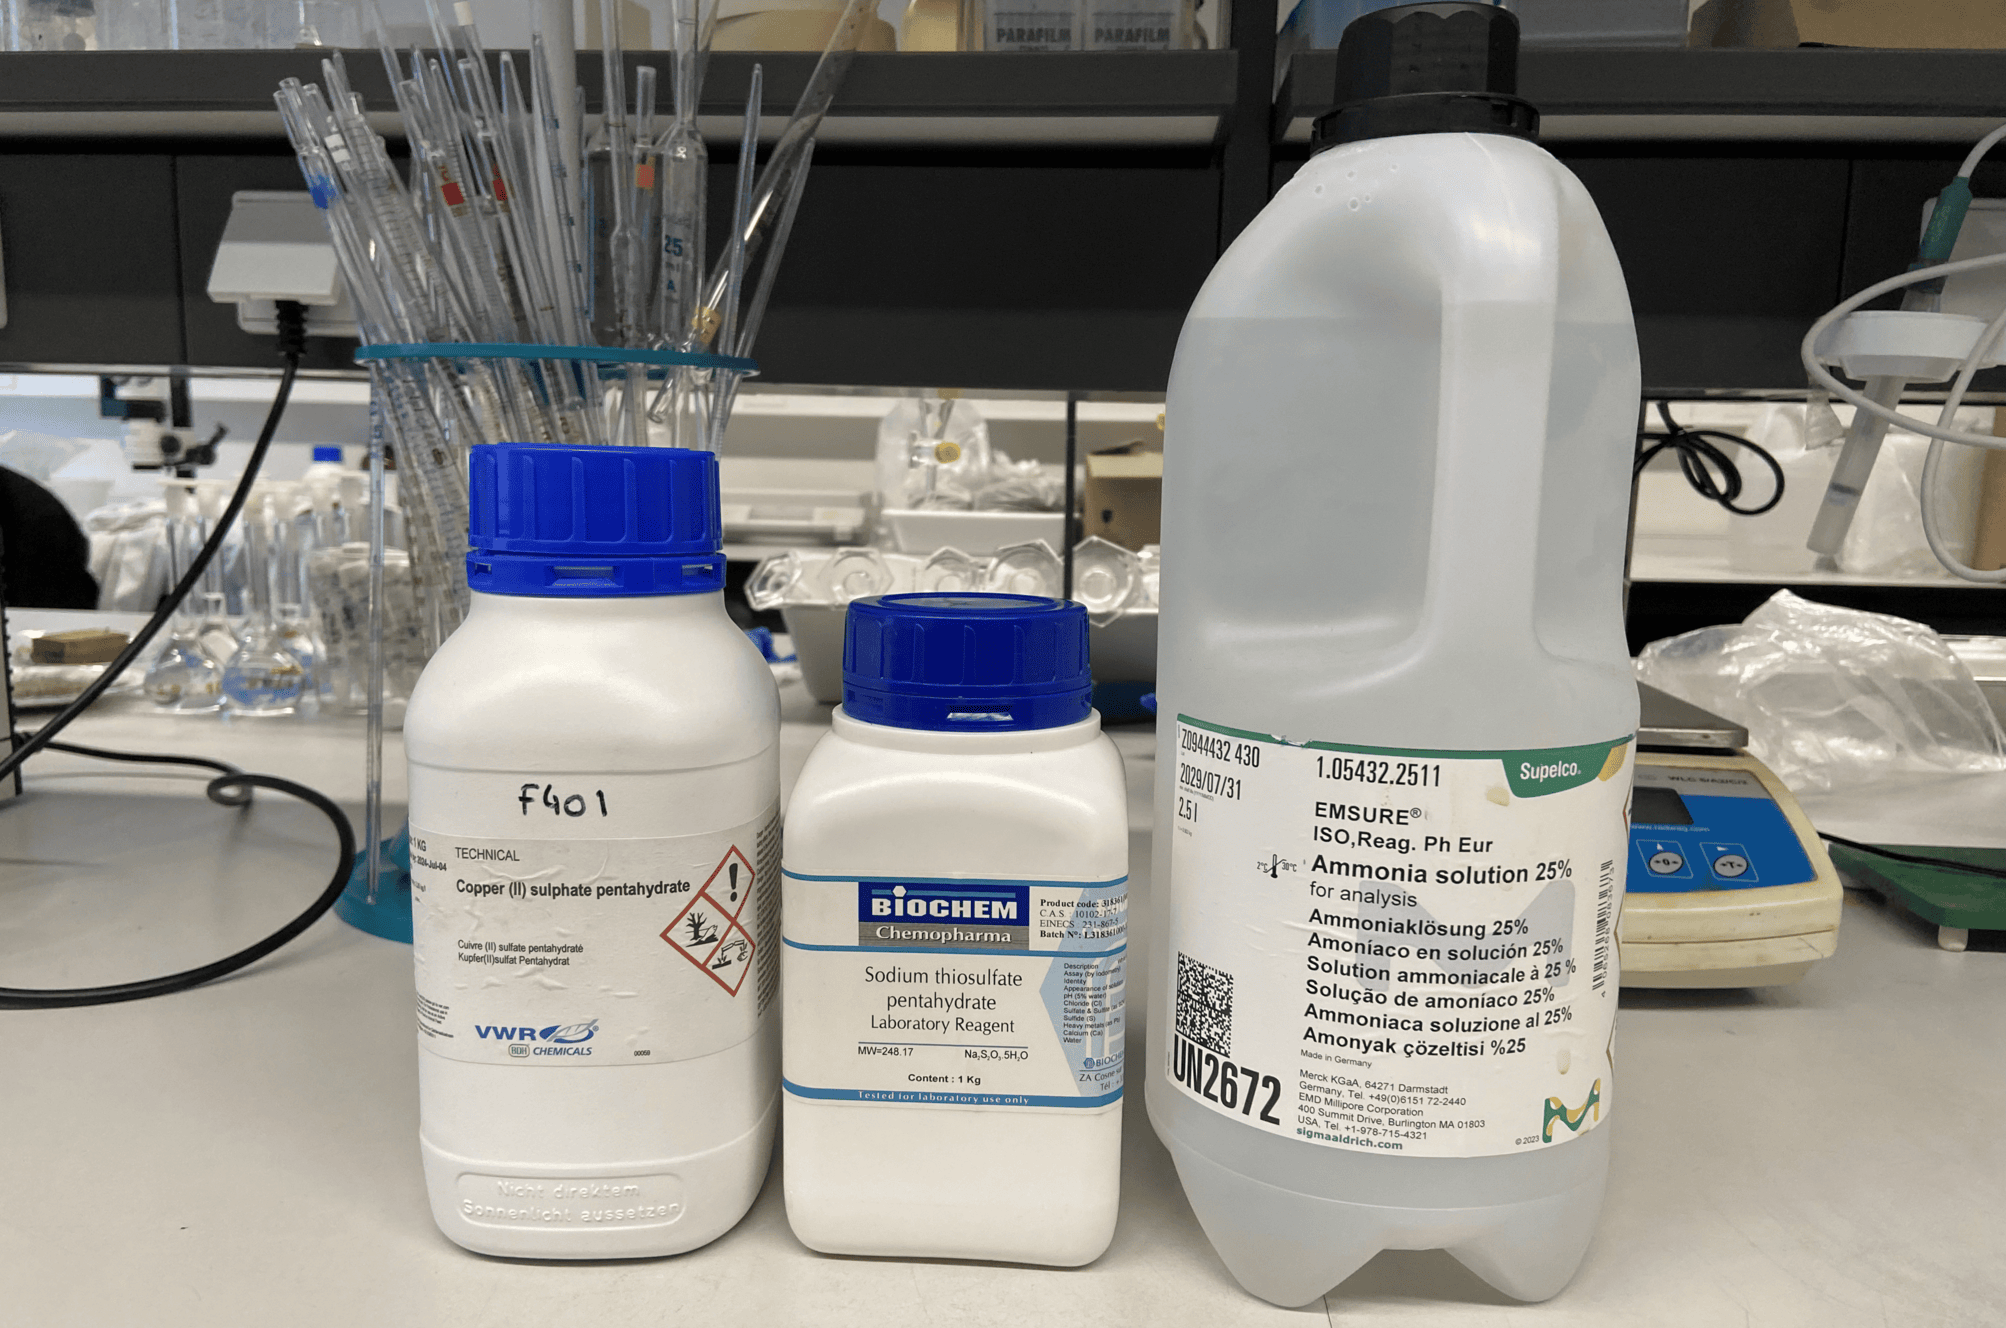
\includegraphics[width=0.9\linewidth]{figures/reagentes-lixiviação 1}
    \caption{Reagentes utilizados na lixiviação.}
    \label{fig:reagentes-lixiviacao-1}
\end{marginfigure}

Num balão volumétrico de 250~mL foi colocado 15~mL de \AMO{}, com uma pipeta de 10~mL\@.
O volume restante foi preenchido com água destilada, até perfazer os 250~mL do balão.
Num gobelé, foi medida a massa de \TSP{} (99,34~g) e a massa de \SCP{} (1,01~g) que vão ser utilizados.
De seguida, juntou-se os conteúdos do balão volumétrico (água + \AMO{}) ao gobelé com o \TSP{} e \SCP{}, agitou-se com uma vareta de vidro até estar bem dissolvido e homogeneizado.

Foi medida a massa de minério a ser lixiviado (200,00~g), da amostra \texttt{A08.3}.
O minério foi colocado dentro do reator de borossilicato.
Adicionou-se ao reator a solução com os reagentes dissolvidos e acrescentou-se 150~mL de água de forma a perfazer os 400~mL de fase líquida, respeitando a relação S/L\@.

\begin{marginfigure}[-8\baselineskip]
    \centering
    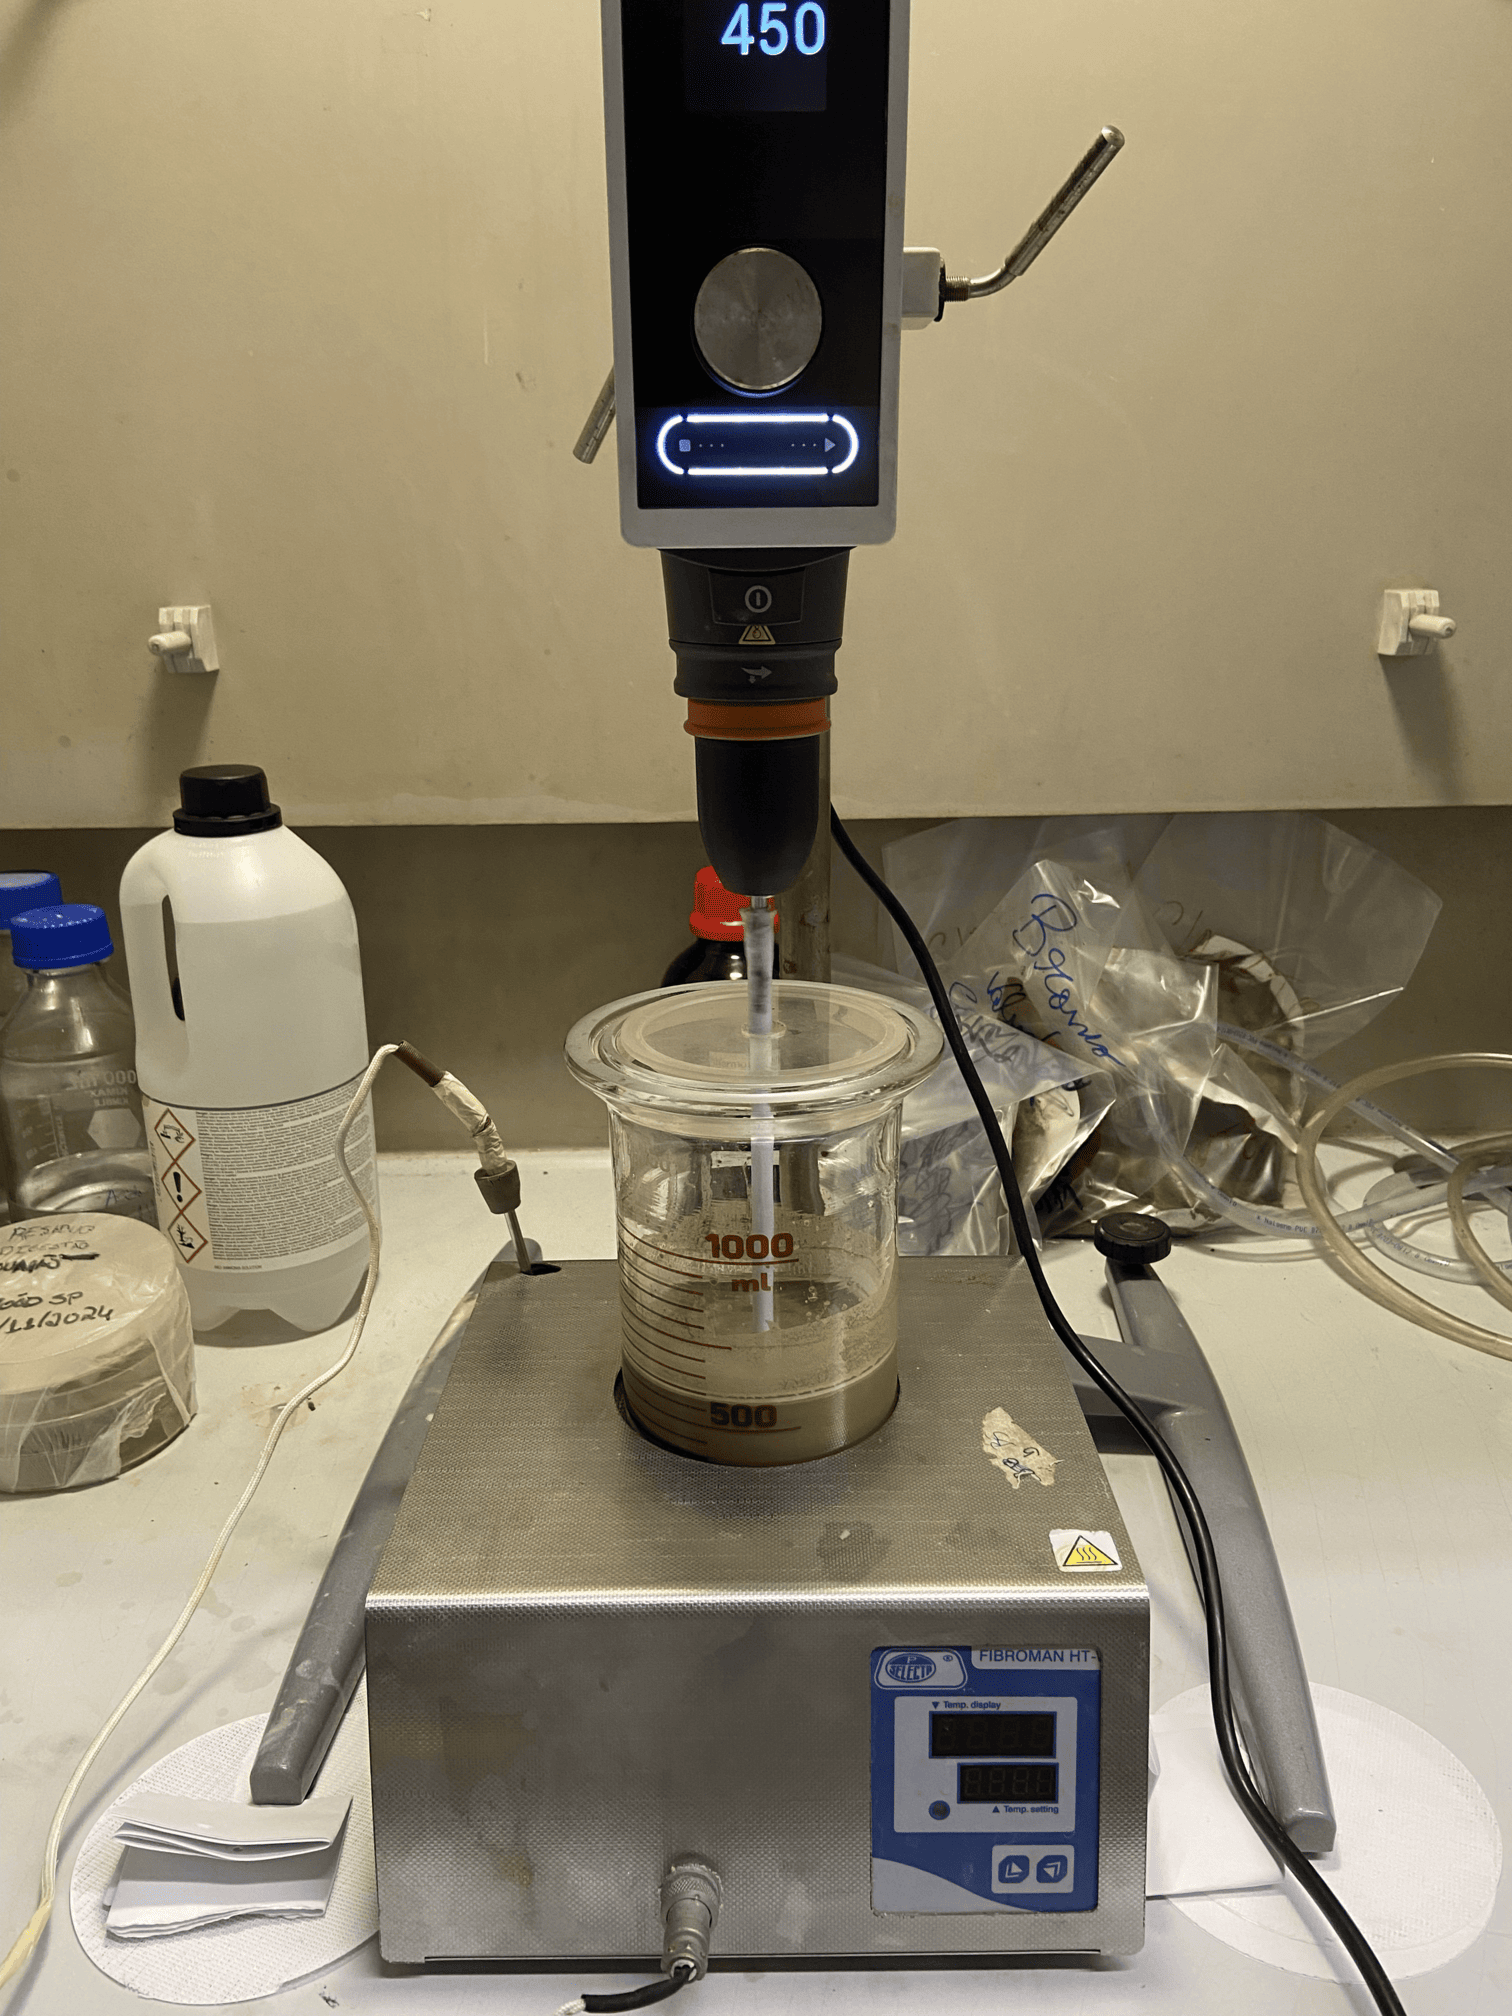
\includegraphics[width=0.9\linewidth]{figures/lixiviação-1 a decorrer}
    \caption{Lixiviação a decorrer.}
    \label{fig:lixiviacao1-a-decorrer}
\end{marginfigure}

Regulou-se o agitador e definiu-se uma velocidade de rotação de 450~rpm.
Deixou-se a trabalhar durante cerca de 5~minutos.
De seguida, parou-se o agitador, deixou-se decantar um pouco e mediu-se o pH (7,25) e o Eh (-86,0~mV - valor medido; 133~mV - valor convertido).

Uma vez registados os valores de pH e Eh, retomou-se o funcionamento do agitador.

\marginnote[-1\baselineskip]{Os valores de pH e de Eh não são fidedignos. Os equipamentos de medição não estavam calibrados, portanto os valores medidos podem não ser os valores reais.}

Deixou-se a lixiviar durante 8~horas.
No fim da lixiviação, mediu-se novamente o pH (6,15) e o Eh (-60,5~mV - valor medido; 159~mV - valor convertido).

De seguida, montou-se o sistema de filtragem, composto por um filtro de Büchner, um Kitasato, uma bomba de vácuo e um papel de filtro.
Filtrou-se e mediu-se o volume do licor de lixiviação - 369~mL\@.

\begin{marginfigure}
    \centering
    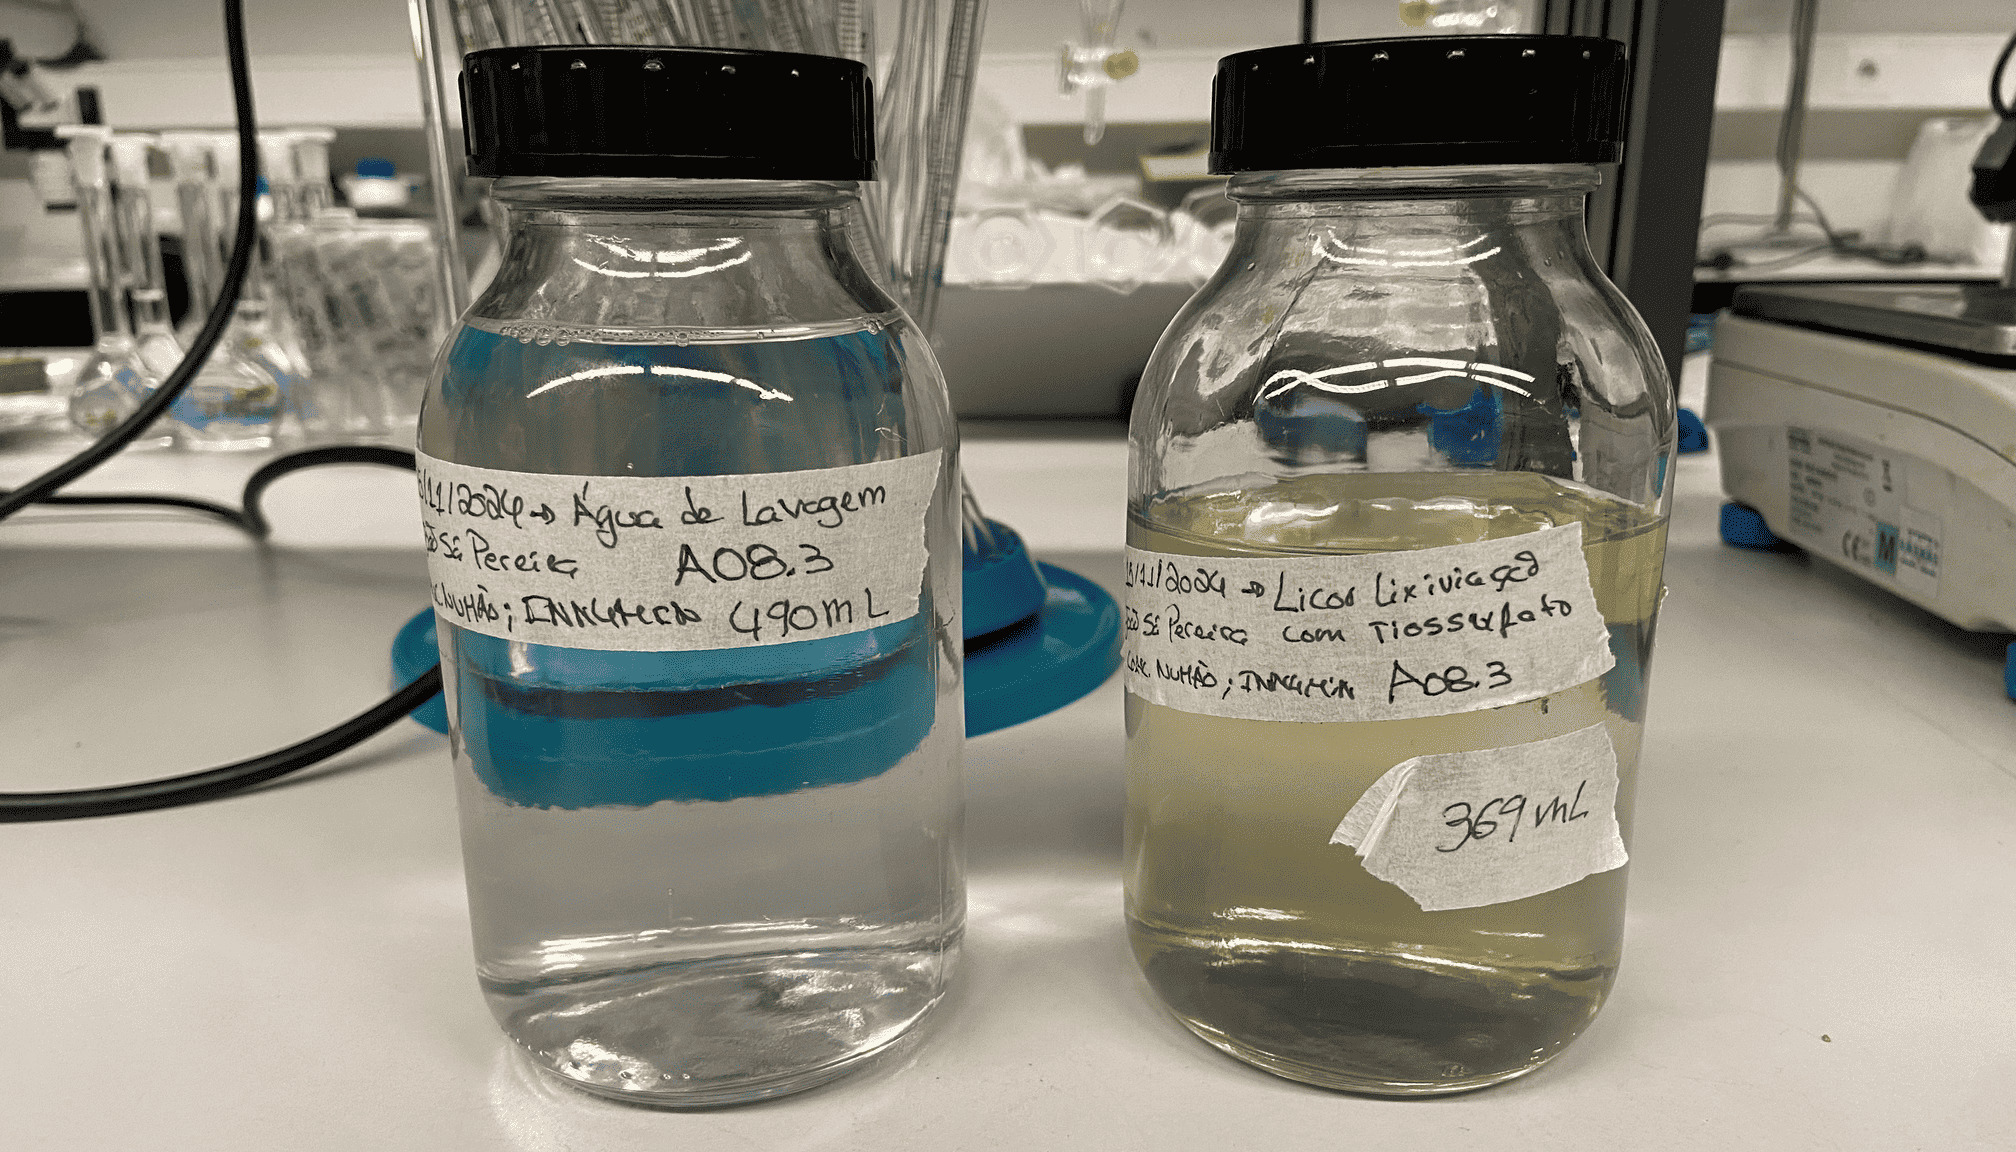
\includegraphics[width=0.9\linewidth]{figures/licor e agua lavagem lix tiossulfato}
    \caption{Licor de lixiviação e água de lavagem (Tiossulfato).}
    \label{fig:licor-lix-agua-lavagem-tiossulfato}
\end{marginfigure}

O resíduo sólido que foi filtrado foi lavado com 500~mL de água.
Colocou-se o resíduo de novo no reator, adicionou-se 500~mL de água e ligou-se o agitador, deixando lavar durante 30~minutos.

Após os 30~minutos, filtrou-se novamente o material.
Mediu-se o volume de solução de água de lavagem - 490~mL\@.

Tanto o licor de lixiviação como a água de lavagem, foram colocados em recipientes de vidro, identificados e armazenados - Figura~\ref{fig:licor-lix-agua-lavagem-tiossulfato}.

\begin{marginfigure}
    \centering
    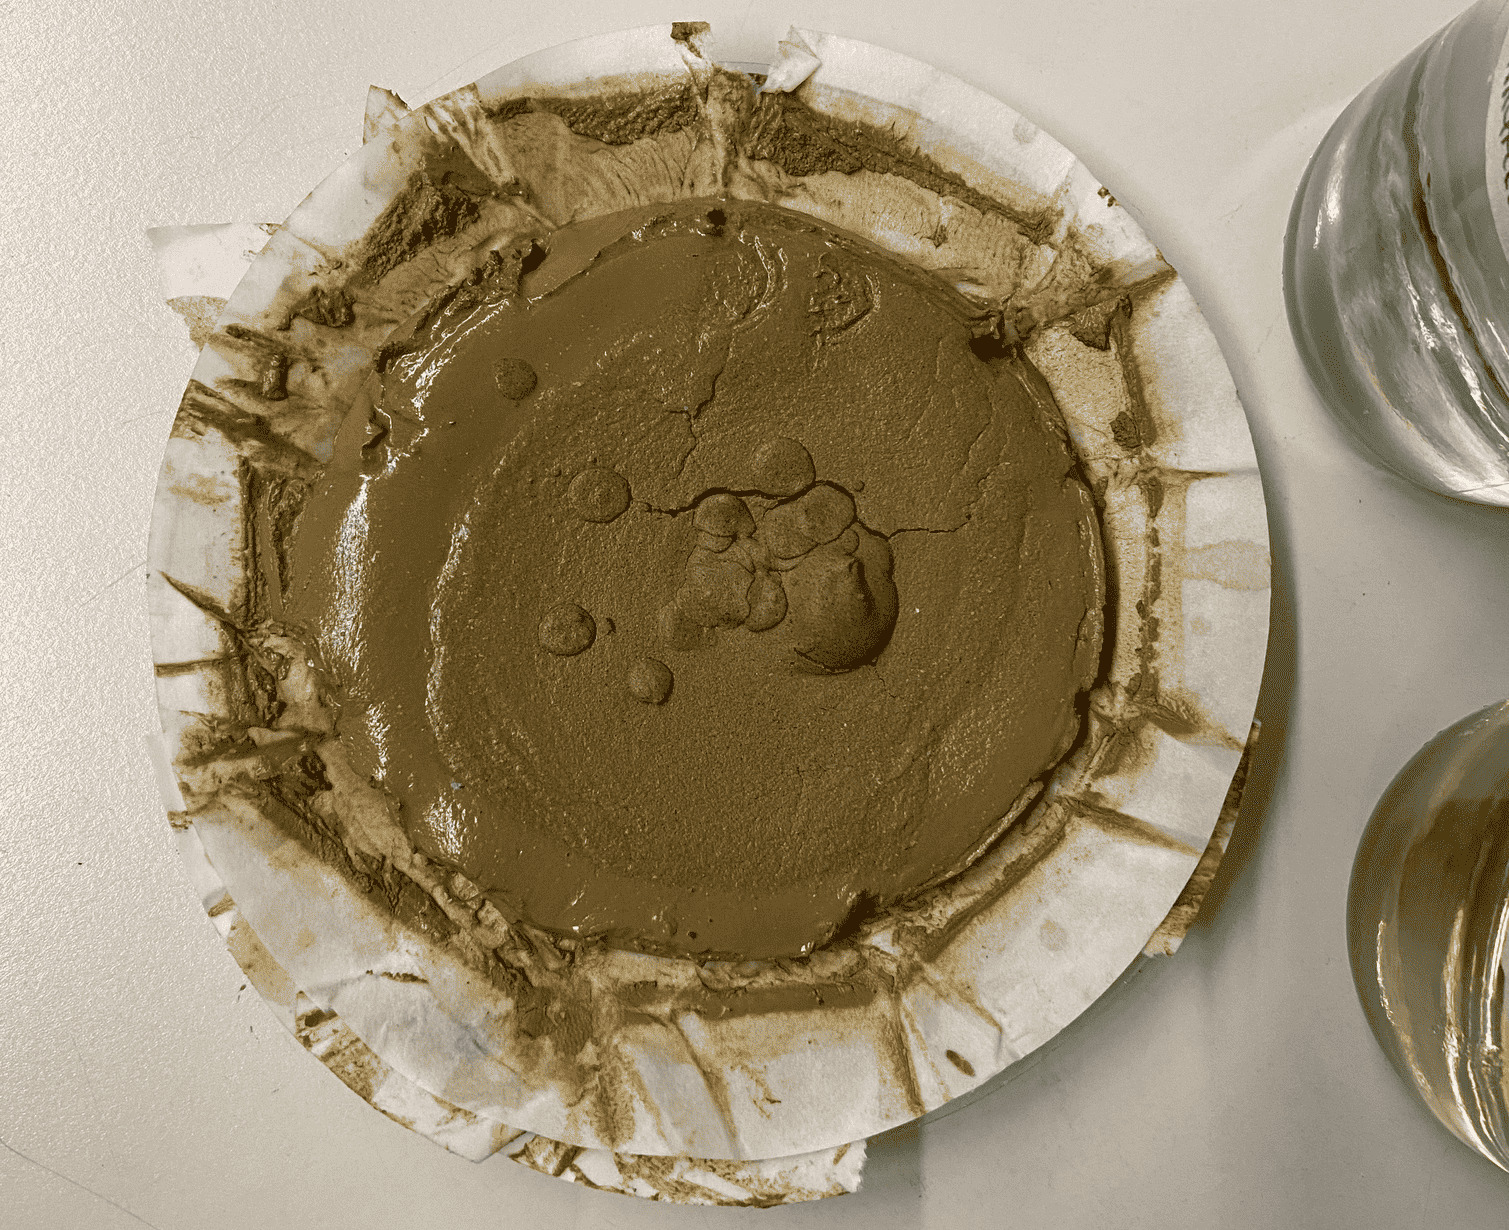
\includegraphics[width=0.9\linewidth]{figures/residuo_sol_lix_tiossulfato}
    \caption{Resíduo sólido da lixiviação (Tiossulfato).}
    \label{fig:res-solido-lix-tiossulfato}
\end{marginfigure}

O material, já lavado e filtrado (Figura~\ref{fig:res-solido-lix-tiossulfato}), foi colocado numa estufa a secar durante o fim-de-semana.
Após estar seco, mediu-se a massa - 192,61~g (já a descontar a massa do vidro de relógio e do papel de filtro).
Reservou-se.

O resíduo sólido será submetido a digestão ácida para análise posterior na absorção atómica.

\newthought{Concentrações em \ce{Au}:} Licor de lixiviação - 1,616~mg/L; água de lavagem - 0,255~mg/L; resíduo (média) - 9,94~ppm.

\hrulefill

%%%%%%%%%%%%%%%%%%%%%%%%%%%%%%%%%%%%%%%%%%%%%%%%%%%%%%%%

\newday{Digestões ácidas dos resíduos de lixiviação - Tiossulfato}

Hoje realizou-se a digestão ácida do resíduo de lixiviação com \TSP{}, do dia~\nameref{day:15-novembro-2024}.

Foi seguido o mesmo procedimento do dia~\nameref{day:8-novembro-2024}.
\marginnote{Ver o procedimento em detalhe para mais informação.}

Utilizou-se a mesma relação de ácido sulfúrico e ácido nítrico, 1:3.
Ou seja, 6~mL de \ce{HNO3} e 18~mL de \ce{HCl}.
Foram feitos 3 ataques, com 1~hora e 30~minutos entre cada um.
Totalizando em 4~horas e 30~minutos de digestão.

No fim dos 3~ataques, juntou-se 4~mL de \ce{HCl} a cada um dos copos e verteu-se para balões volumétricos de 50~ml, separando o resíduo sólido do líquido.
O volume restante dos balões foi preenchido com água destilada.
O resíduo sólido foi colocado numa placa de Petri e reservado.

Posteriormente, o conteúdo dos balões volumétricos será filtrado para ser analisado na absorção atómica.

Após a análise na absorção atómica, obteve-se a Tabela~\ref{tab:aas-concentracao-au-res-tiossulfato} referente às concentrações em Au no resíduo de lixiviação com Tiossulfato:

\begin{table}[!ht]
    \centering
    \begin{tabularx}{\textwidth}{@{}lCCC@{}}
        \toprule
        \textbf{Amostra} & \textbf{Absorção} & \textbf{Conc. (mg/L)} & \textbf{Teor \ce{Au} (ppm)} \\ \midrule
        \textbf{Dig. 1} & 0,06004 & 1,96 & 9,8221 \\
        \textbf{Dig. 2} & 0,06407 & 2,09 & 10,4402 \\
        \textbf{Dig. 3} & 0,06463 & 2,11 & 10,5261 \\
        \textbf{Dig. 4} & 0,05436 & 1,79 & 8,9509 \\
        \textbf{Dig. 5} & 0,06083 & 1,99 & 9,9433 \\ \bottomrule
    \end{tabularx}
    \caption{Concentração em \ce{Au} no resíduo de lixiviação com Tiossulfato.}
    \label{tab:aas-concentracao-au-res-tiossulfato}
\end{table}

Da absorção atómica também se determinou a concentração em \ce{Au} do licor de lixiviação (\textbf{1,616~mg/L}) e da água de lavagem (\textbf{0,255~mg/L}).

\hrulefill

%%%%%%%%%%%%%%%%%%%%%%%%%%%%%%%%%%%%%%%%%%%%%%%%%%%%%%%%

\newday{22 Novembro 2024}\label{day:22-novembro-2024}

Hoje realizou-se a lixiviação com \textbf{Tioureia} (\tioureia{}) de um dos restantes sacos de $\approx$~250~g da amostra \texttt{A08}.
O saco selecionado, aleatoriamente, foi a sub-amostra \texttt{A08.4}.

Para a elaboração do procedimento desta lixiviação, foi tomado em consideração o artigo ``\emph{An innovative thiourea gold leaching process}''\cite{innovative_thiourea_1998}.
A partir deste artigo foram definidas as concentrações dos reagentes a usar e o procedimento a ser tomado para a lixiviação.

Nesse sentido, as concentrações utilizadas foram as seguintes:
\begin{itemize}
    \item[-] Tioreia, \tioureia{} - 100~g/kg de minério;
    \item[-] Sulfato de ferro (III) penta-hidratado, \sulfe{}: 0,5~g/kg de minério;
    \item[-] Ácido sulfúrico, \acsul{} - o necessário para obter uma solução com pH = 1.
\end{itemize}

Foi decidido utilizar 100~g de minério da sub-amostra \texttt{A08.4}, para a lixiviação. 
A lixiviação será feita com uma razão sólido líquido de 1 para 5 (S/L = 1/5).

A lixiviação foi efetuada a temperatura ambiente, com uma agitação de 350~rpm, durante 6~horas.
Foi utilizado um reator de borossilicato de 500~mL.

Foi realizado o cálculo da quantidade de reagentes necessários, para as concentrações estipuladas. 
Para o caso do sulfato de ferro (III), como a concentração utilizada no artigo era muito baixa, utilizou-se sulfato de ferro (III) penta-hidratado. Portanto, ajustou-se os cálculos tendo em consideração esta alteração.

A quantidade de reagentes utilizada foi a seguinte:
\begin{itemize}
    \item[-] $\mathrm{m}_{\left[\tioureia{}\right]}$ = 10~g;
    \item[-] $\mathrm{m}_{\left[\sulfe{}\right]}$ = 0,0612~g;
    \item[-] $\mathrm{V}_{\left[\acsul{}\right]}$ = 1,85~mL.
\end{itemize}

\marginnote[-1cm]{O ácido sulfúrico foi adicionado, pouco a pouco, no reator em agitação com apenas tioureia dissolvida. Foi-se medindo o pH à medida que se ia adicionando \acsul{} até que a solução se apresentou com pH de 1,3.}

No reator de borossilicato, foi adicionado 500~mL de água destilada e 10~g de \tioureia{}   .
Dissolveu-se a tioureia com auxílio do agitador mecânico e ajustou-se o pH, adicionando 1,85~ml de \acsul{}, o que resultou num pH = 1,3.
Após acidificar a solução, adicionou-se \sulfe{} e o minério no reator, regulando o agitador para 350~rpm e dando início à lixiviação às 10h18.

Foi-se verificando o pH ao longo da lixiviação para garantir que a solução se encontrava com um pH = 1, adicionando \acsul{} conforme necessário.

\begin{marginfigure}
    \centering
    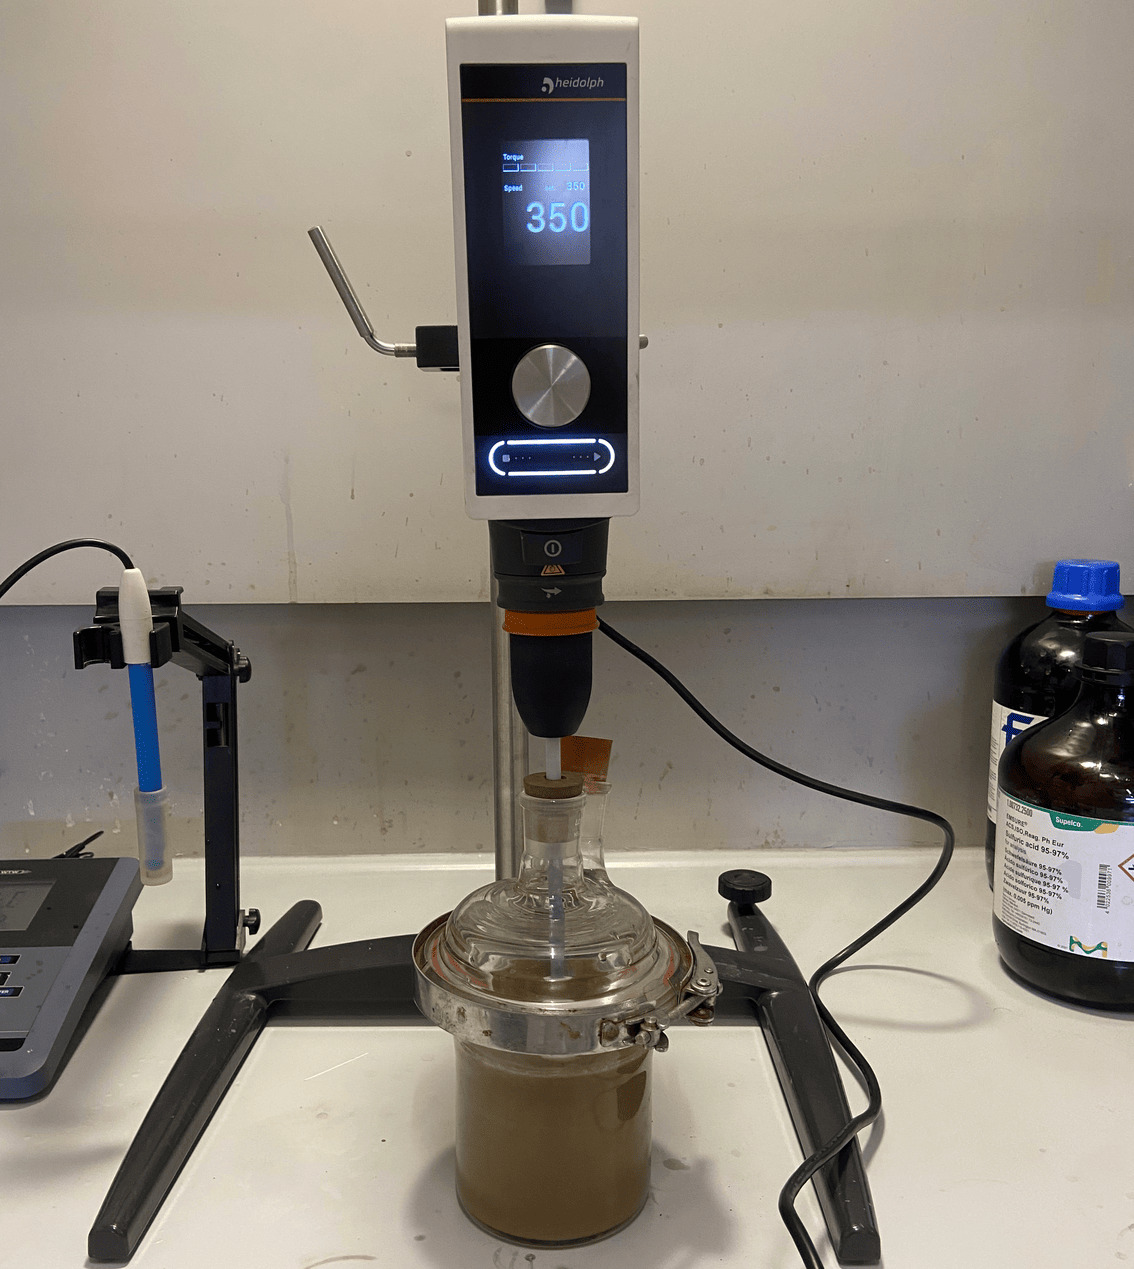
\includegraphics[width=0.9\linewidth]{figures/Lixiviação - Tioureia}
    \caption{Lixiviação com tioureia a decorrer.}
    \label{fig:lix-tioureia-a-decorrer}
\end{marginfigure}

Adicionou-se, durante as 6~horas de lixiviação, 1,465~mL de \acsul{}.
No total adicionou-se 3,315~mL de \acsul{}, sendo que 1,85~mL foi adicionado antes da lixiviação, sem o minério na solução e 1,465~mL foi adicionado durante a lixivição, com o minério na solução.

Foi preparada uma solução de lavagem com água destilada acidificada (pH = 1).
A relação S/L para a lavagem foi de 1/2,5. 
Portanto, para 100~g de minério utilizou-se 250~mL de água destilada acidificada.
Para acidificar 250~mL de água destilada, adicionou-se 1~mL de \acsul{} resultando num pH = 1,046.

Uma vez terminada a lixiviação, filtrou-se o material com um sistema de filtração composto por um filtro Büchner, um balão Kitasato, um papel de filtro e uma bomba de vácuo. 
Filtrou-se a solução, mediu-se o volume de licor filtrado (473~mL) e mediu-se o pH do licor (1,195).

\begin{marginfigure}
    \centering
    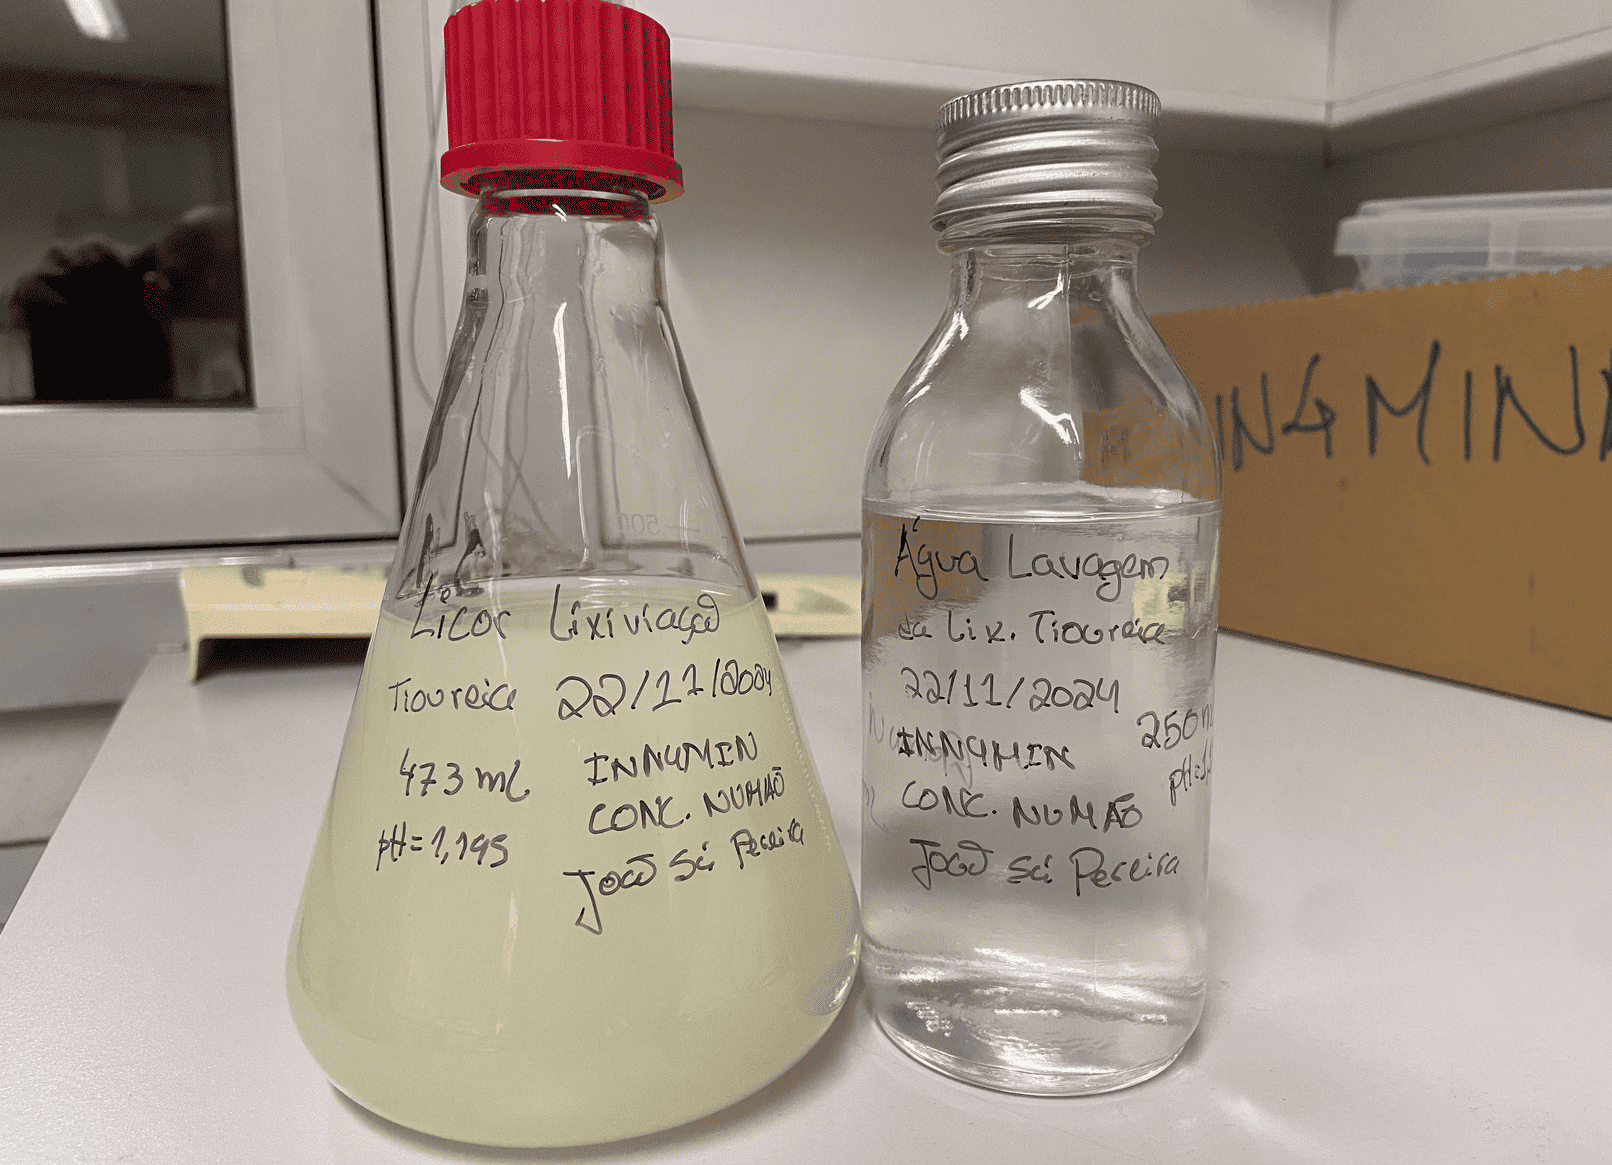
\includegraphics[width=0.9\linewidth]{figures/Lixiviação Tioureia (Licor e Água de Lavagem)}
    \caption{Licor de lixiviação e água de lavagem (Tioureia).}
    \label{fig:licor-agualavagem-tioureia}
\end{marginfigure}

Colocou-se o sólido filtrado novamente no reator de borossilicato, adicionou-se os 250~mL de água destilada acidificada e deixou-se a lavar durante 30~minutos com o agitador mecânico a 350~rmp.
Uma vez terminada a lavagem, filtrou-se novamente com o mesmo sistema de filtragem.
Mediu-se o volume da água de lavagem (250~mL) e mediu-se o pH (1,118).

Tanto o licor de lixiviação como a água de lavagem, foram colocados em recipientes de vidro, identificados e armazenados - Figura~\ref{fig:licor-agualavagem-tioureia}.

O sólido filtrado foi colocado numa placa de Petri e deixado a secar na estufa a 60~\graus{} durante 8~horas.
O resíduo sólido ficou dentro da estufa (desligada), durante o fim de semana.
O papel de filtro utilizado nas duas filtragens, pesavam 2,40~g e 2,33~g\sidenote{Não esquecer de remover estes valores quando se for medir a massa do resíduo sólido seco.}.

Após estar seco, mediu-se a massa - 86,2~g (já a descontar a massa do vidro de relógio e do papel de filtro). 
Reservou-se.

O resíduo sólido será submetido a digestão ácida para análise posterior na absorção atómica.

\newthought{O licor de lixiviação e a água de lavagem} precipitaram material durante os dias em que não foram analisados.
Portanto, antes de se efetuar a análise por absorção atómica, deverá ser filtrado tanto o licor de lixiviação como a água de lavagem. 
O resíduo precipitado será armazenado para posterior análise no FRX.

\newthought{Concentrações em \ce{Au}:} Licor de lixiviação - 1,108~mg/L; água de lavagem - 0,1071~mg/L; resíduo (média) - 8,71~ppm.

\hrulefill

%%%%%%%%%%%%%%%%%%%%%%%%%%%%%%%%%%%%%%%%%%%%%%%%%%%%%%%%

\newday{Digestões ácidas dos resíduos de lixiviação - Tioureia}

Hoje realizaram-se as digestões ácidas do resíduo sólido proveniente da lixiviação com tioureia, do dia~\nameref{day:22-novembro-2024}.

O procedimento seguido para a preparação da amostra para ser colocada na mufla e da digestão ácida em si foi os do dia~\nameref{day:7-novembro-2024} e \nameref{day:8-novembro-2024}, respetivamente.

Após a análise na absorção atómica, obteve-se a Tabela~\ref{tab:aas-concentracao-au-res-tioureia} referente às concentrações em \ce{Au} no resíduo de lixiviação com Tioureia.

\begin{table}[!ht]
    \centering
    \begin{tabularx}{\textwidth}{@{}lCCC@{}}
        \toprule
        \textbf{Amostra} & \textbf{Absorção} & \textbf{Conc. (mg/L)} & \textbf{Teor \ce{Au} (ppm)} \\ \midrule
        \textbf{Dig. 1} & 0,06242 & 2,04 & 10,2000 \\
        \textbf{Dig. 2} & 0,04530 & 1,51 & 7,5500 \\
        \textbf{Dig. 3} & 0,05001 & 1,66 & 8,3000 \\
        \textbf{Dig. 4} & 0,05425 & 1,79 & 8,9500 \\
        \textbf{Dig. 5} & 0,05173 & 1,71 & 8,5500 \\ \bottomrule
    \end{tabularx}
    \caption{Concentração em \ce{Au} no resíduo de lixiviação com Tioureia.}
    \label{tab:aas-concentracao-au-res-tioureia}
\end{table}

Da absorção atómica também se determinou a concentração em \ce{Au} do licor de lixiviação (\textbf{1,108~mg/L}) e da água de lavagem (\textbf{0,1071~mg/L}).

\hrulefill

%%%%%%%%%%%%%%%%%%%%%%%%%%%%%%%%%%%%%%%%%%%%%%%%%%%%%%%%

\newday{27 Novembro 2024}\label{day:27-novembro-2024}

Hoje realizou-se a lixiviação com \textbf{Brometo de Sódio}, \bromo{}, de um dos restantes sacos de $\approx$~250~g.
O saco selecionado, aleatoriamente, foi a sub-amostra \texttt{A08.1}.

Para a elaboração do procedimento desta lixiviação, foi tomado em consideração o artigo ``\emph{Bromine leaching as an alternative method for gold dissolution}''~\cite{bromo_2018}.
A partir deste artigo foram definidas as concentrações dos reagentes a usar e o procedimento a ser tomado para a lixiviação.

Nesse sentido as concentrações utilizadas foram as seguintes:
\begin{itemize}
    \item[-] Brometo de sódio, \bromo{} = 0,43~M ou 44~g/L;
    \item[-] Ácido clorídrico a 37~\%, \acl{} = 0,42~M;
    \item[-] Hipoclorito de sódio, \hipso{} = 0,23~M.  
\end{itemize}

Utilizou-se 200~g de minério da amostra \texttt{A08.1}, para a lixiviação.
A lixiviação foi realizada com uma razão sólido líquido de 1 para 1 (S/L = 1/1).

A lixiviação foi efetuada a 60~\graus{}, em banho maria, com uma agitação de 400~rpm, durante 6~horas.
Foi utilizado um reator de borossilicato de 500~mL.

Foram realizados os cálculos das quantidades de reagentes necessários, para as concentrações estipuladas. 

A quantidade de reagentes utilizada foi a seguinte:
\begin{itemize}
    \item[-] $\mathrm{m}_{\left[\bromo{}\right]}$ = 8,8~g;
    \item[-] $\mathrm{V}_{\left[\acl{}\right]}$ = 2,57~mL;
    \item[-] $\mathrm{V}_{\left[\hipso{}\right]}$ = 22,8~mL.
\end{itemize}

\begin{marginfigure}
    \centering
    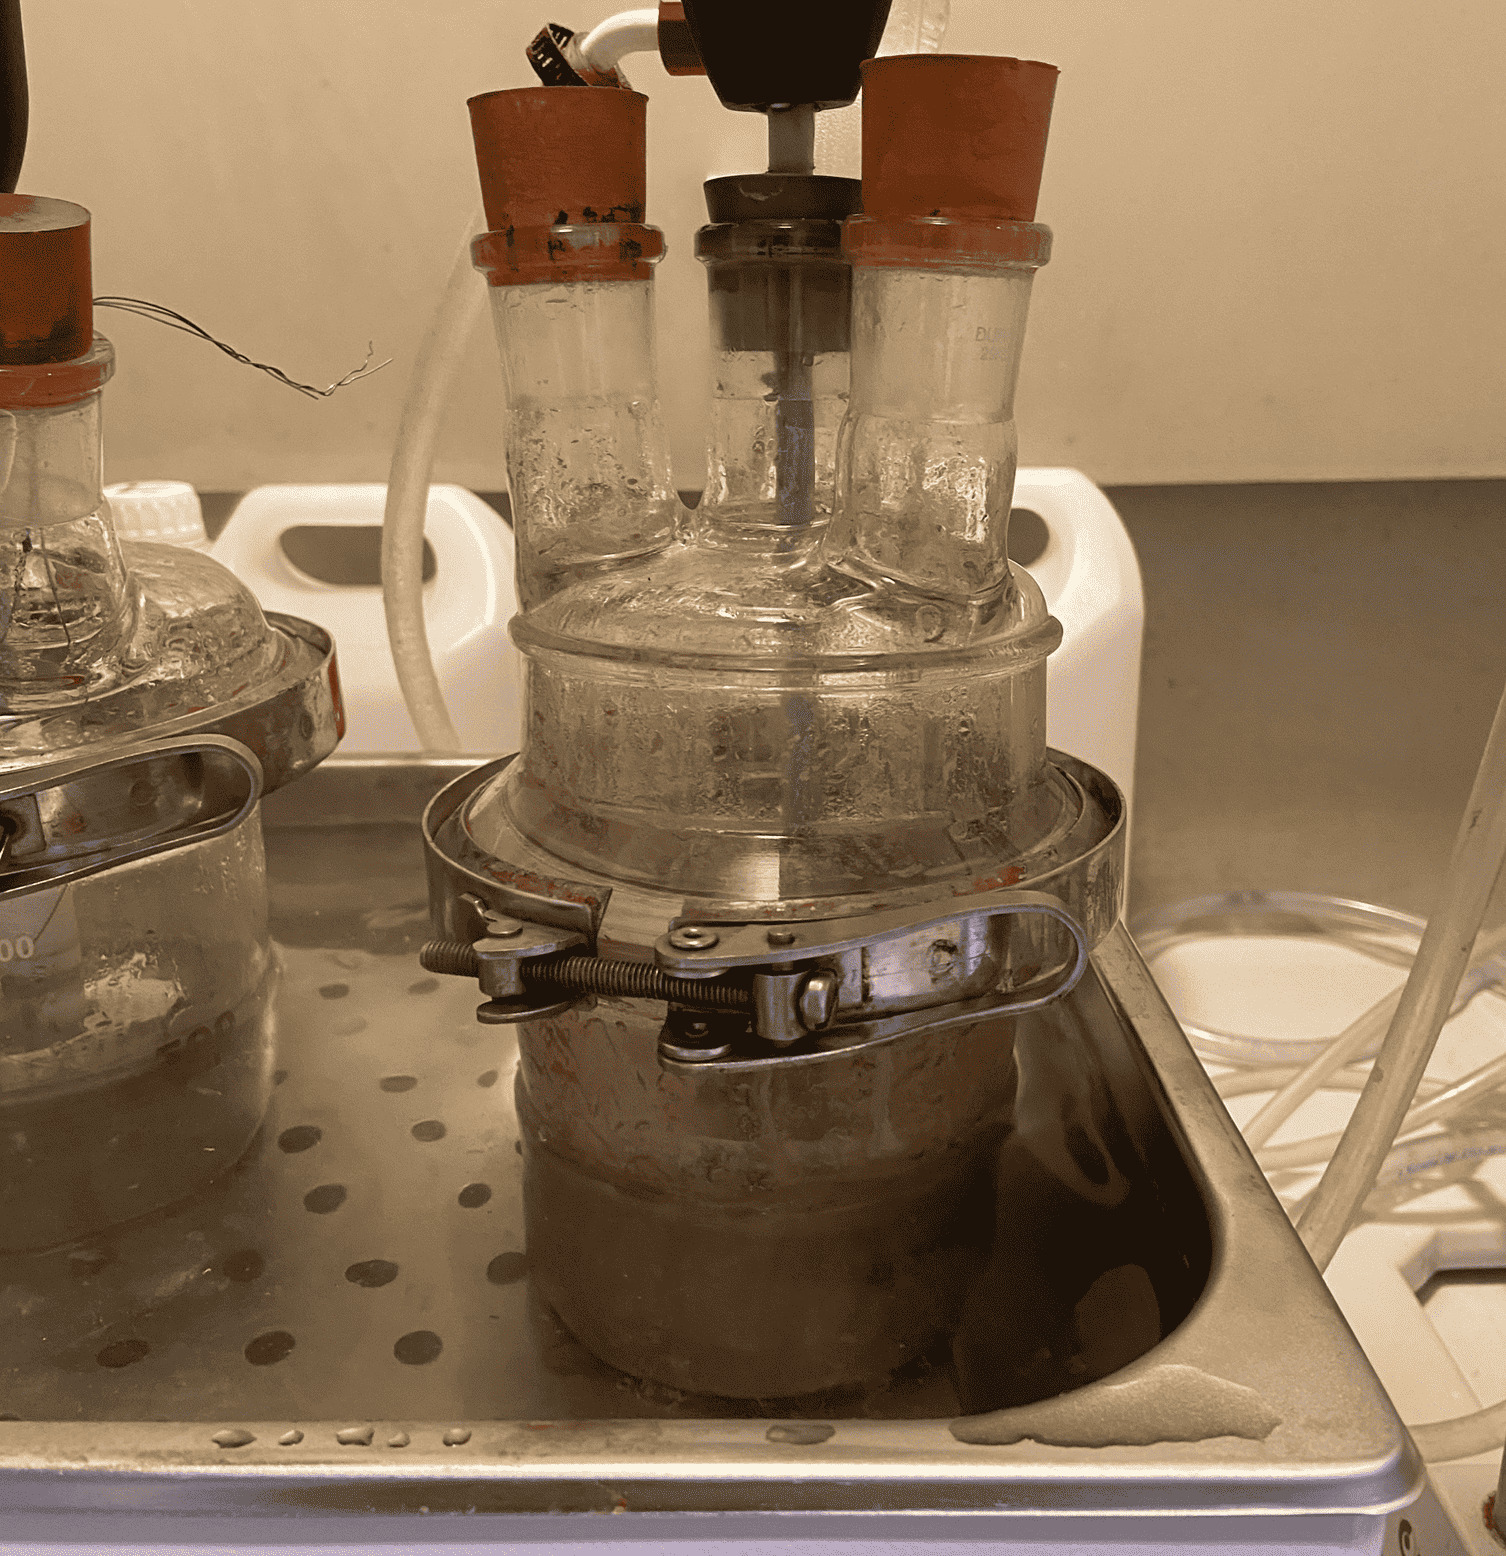
\includegraphics[width=0.9\linewidth]{figures/lixiviação bromo}
    \caption{Lixiviação com Bromo a decorrer.}
    \label{fig:lixiacao-bromo}
\end{marginfigure}

Numa proveta de 250~mL, foi adicionado cerca de 100~mL de água destilada.
De seguida, com uma pipeta de 1~mL, foi adicionado 2,57~mL de \acl{} a 37~\%.
Depois, com uma pipeta de 10~mL, foi adicionado 22.8~mL de \hipso{}.

Montou-se o reator de borossilicato, com 4 aberturas. 
Numa das aberturas, colocou-se a coluna de condensação. 
Noutra abertura colocou-se o agitador mecânico.
As outras duas aberturas permaneceram seladas, sendo utilizadas apenas para adicionar o \bromo{} e para medir o pH, quando necessário.

\marginnote{Adicionou-se o \bromo{} em último para que quando fosse adicionado se pudesse selar o reator imediatamente, de forma a evitar fugas de bromo.}

Uma vez montado o reator, adicionou-se 200~g de minério.
Selou-se o reator.
Adicionou-se a solução acidificada com ácido clorídrico e hipoclorito de sódio.
Apenas depois de se ter adicionado tudo, é que se adicionou o brometo de sódio.
Regulou-se a agitação para 400~rpm\sidenote{No protocolo estava estipulado uma velocidade de rotação de 450~rpm, mas com esta velocidade o sistema reator + agitador + banho maria tornava-se muito instável. Portanto, reduziu-se a velocidade o que melhorou a estabilidade.} e deixou-se a trabalhar durante 5~minutos.
Após os 5~minutos, mediu-se rapidamente o pH (0,231) para evitar fugas de bromo.
Deixou-se a lixiviação decorrer durante as 6~horas, verificando periodicamente a estabilidade do reator.

Uma vez terminada a lixiviação, filtrou-se o material com um sistema de filtração composto por um filtro de Büchner, um balão Kitasato, um papel de filtro e uma bomba vácuo.
Filtrou-se a solução, mediu-se o volume de licor filtrado (93~mL) e mediu-se o pH do licor (0,934).

Colocou-se o sólido filtrado novamente no reator de borossilicato, adicionou-se 500~mL de água destilada e deixou-se a lavar durante 30~minutos com o agitador mecânico regulado a 400~rpm.
Uma vez terminada a lavagem, filtrou-se novamente com o mesmo sistema de filtragem.
Mediu-se o volume de água de lavagem filtrada (480~mL) e mediu-se o pH (2,034).

Tanto o licor como a água de lixiviação, foram colocados em recipientes de vidro, identificados e armazenados.

O sólido lavado e filtrado foi colocado numa placa de Petri na estufa e deixado a secar a 60~\graus{} durante 8~horas, sendo que após este tempo ficou dentro da estufa durante a noite.

Após estar seco (Figura~\ref{fig:residuo-solido-bromo}), mediu-se a massa - 181,98~g (já a descontar a massa do vidro de relógio e do papel de filtro).
Reservou-se.

\begin{marginfigure}[-1cm]
    \centering
    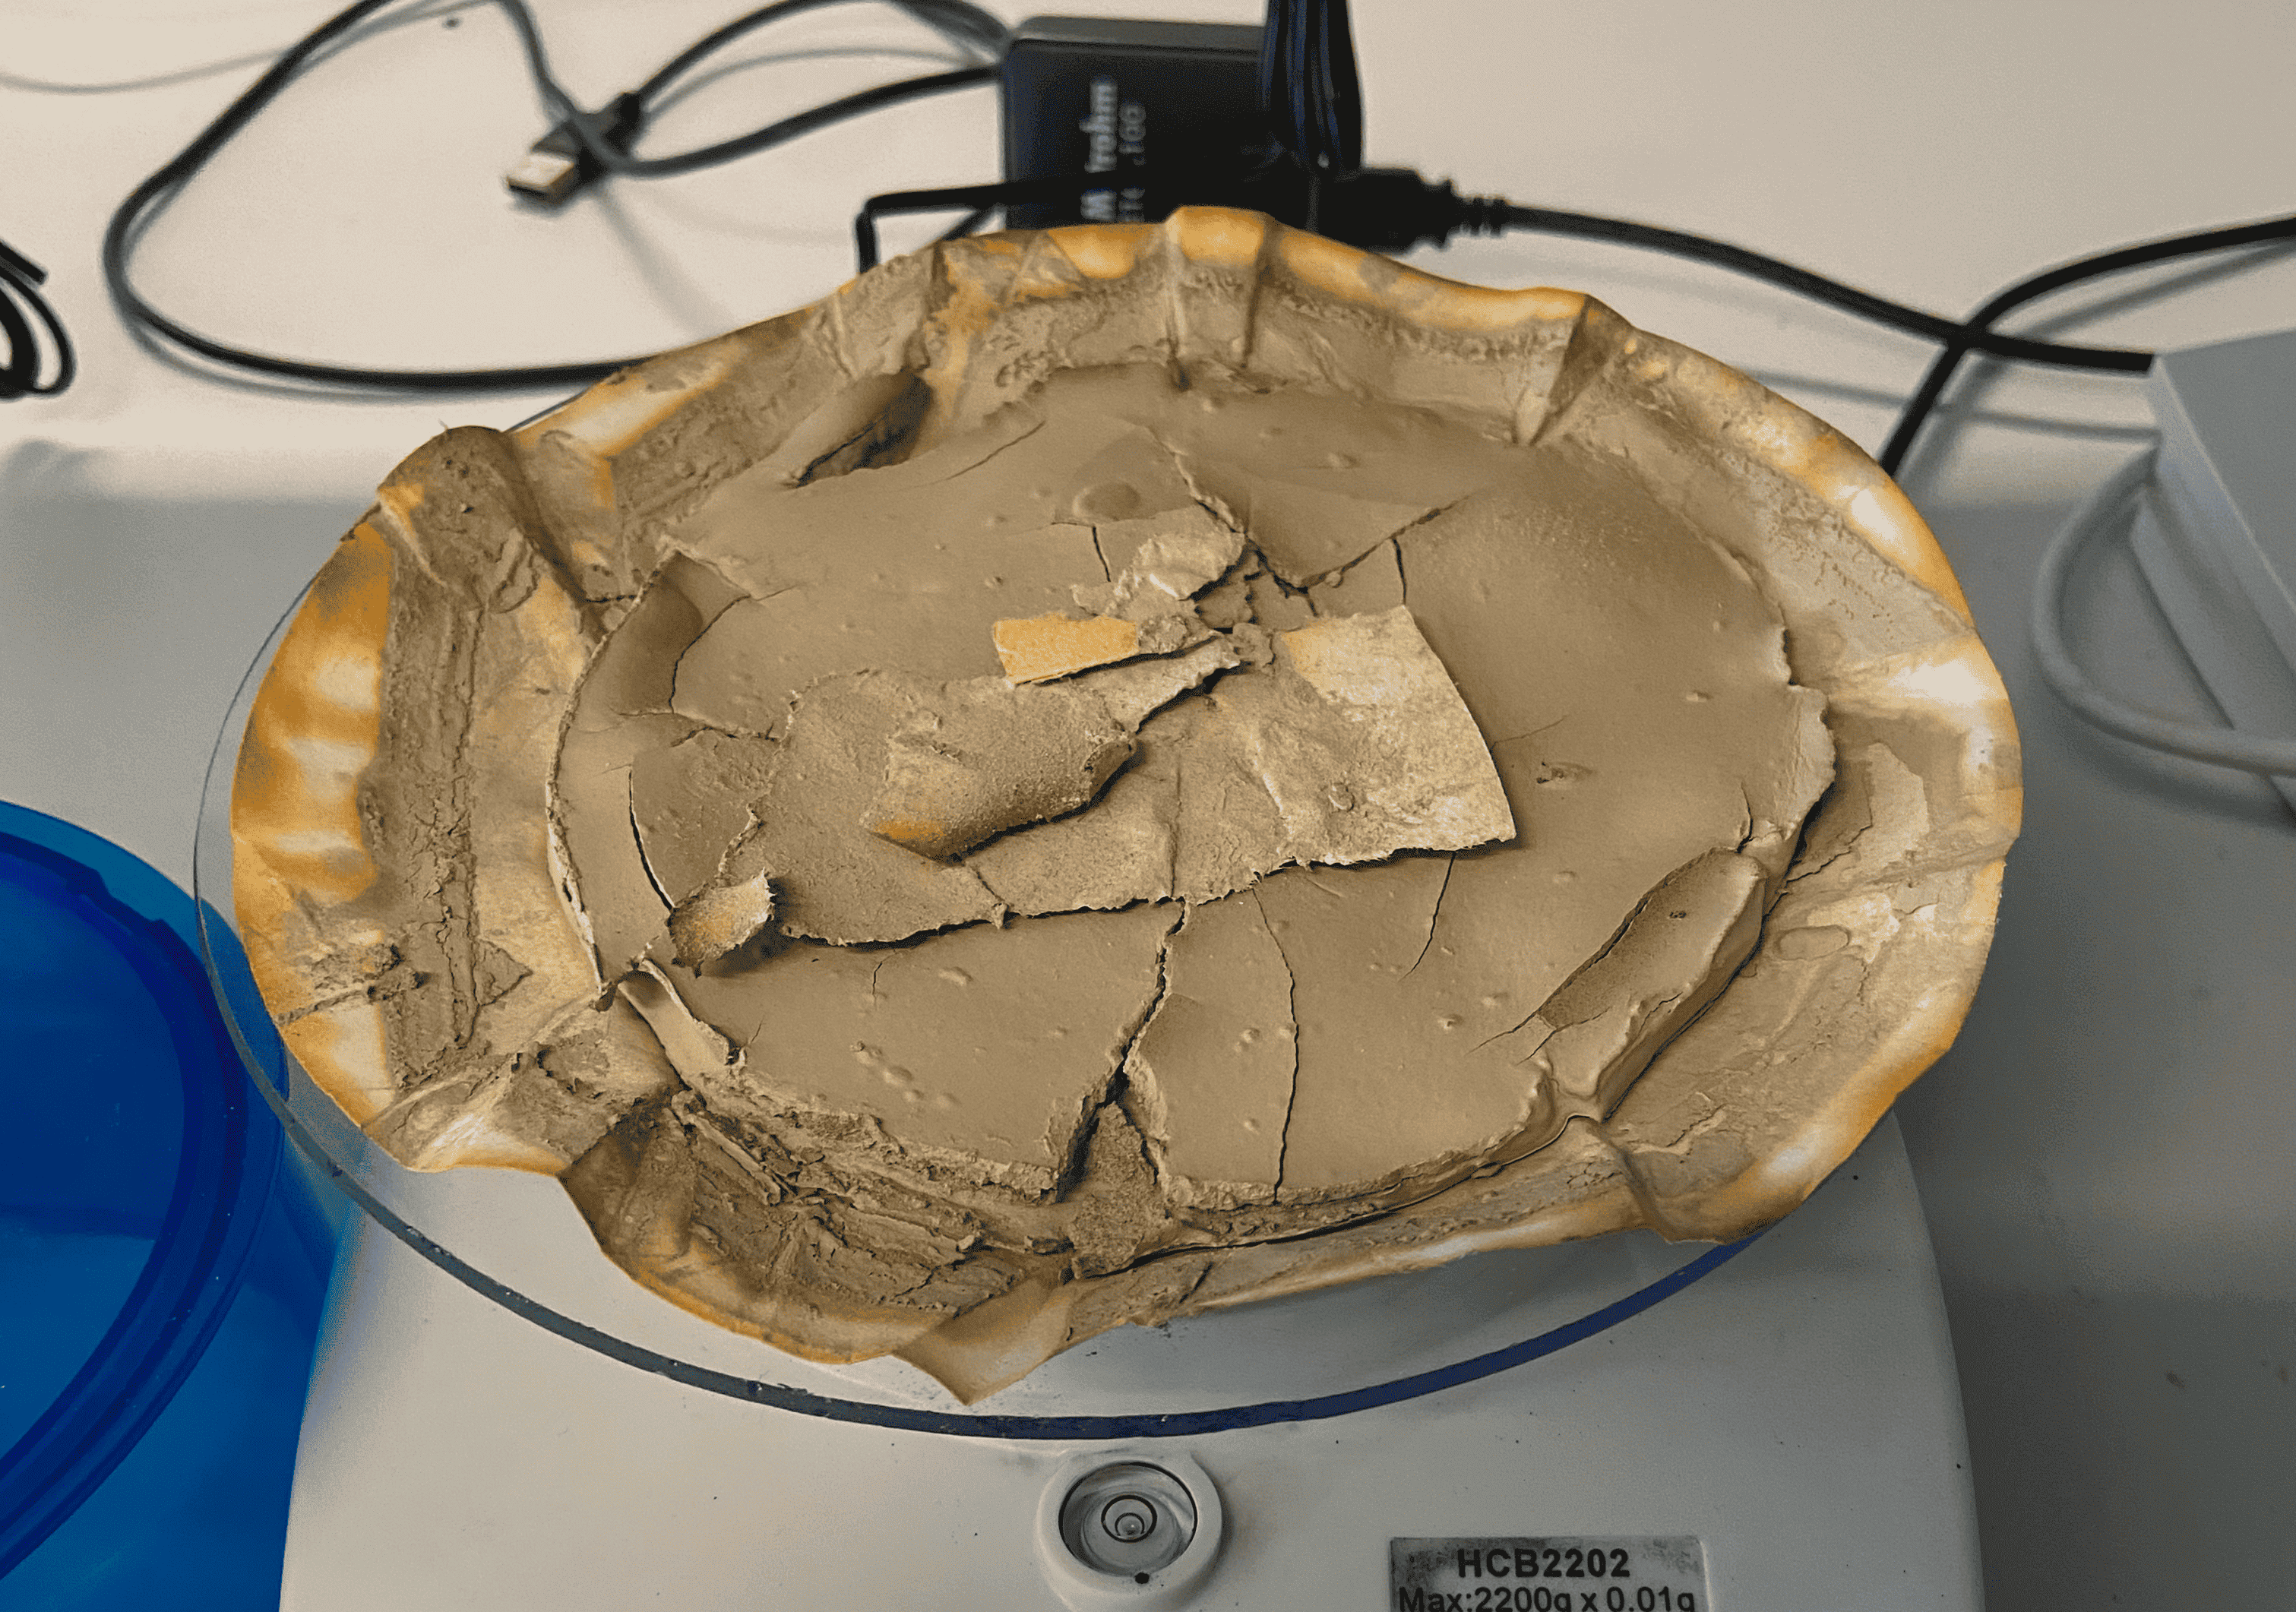
\includegraphics[width=0.9\linewidth]{figures/residuo solido lavado e filtrado - bromo}
    \caption{Resíduo sólido lavado e filtrado, seco (Bromo).}
    \label{fig:residuo-solido-bromo}
\end{marginfigure}

O resíduo sólido será submetido a digestão ácida para análise posterior na absorção atómica.

\newthought{Concentrações em \ce{Au}:} Licor de lixiviação - 3,694~mg/L; água de lavagem - 0,512~mg/L; resíduo (média) - 9,13~ppm.

\hrulefill

\newday{Digestões ácidas dos resíduos de lixiviação - Bromo}

Após se realizar as digestões ácidas\sidenote{O procedimento para a digestão ácida foi o mesmo realizado no dia~\nameref{day:8-novembro-2024}.} do resíduo sólido lixiviado com brometo de sódio, analisou-se na absorção atómica.

Após a análise na \emph{AAS}, obteve-se a Tabela~\ref{tab:aas-concentracao-au-res-bromo} referente às concentrações em \ce{Au} no resíduo de lixiviação com brometo de sódio.

Da absorção atómica também se determinou a concentração em \ce{Au} do licor de lixiviação (\textbf{3,694~mg/L}) e da água de lavagem (\textbf{0.512~mg/L}).

\newpage

\begin{table}[!ht]
    \centering
    \begin{tabularx}{\textwidth}{@{}lCCC@{}}
        \toprule
        \textbf{Amostra} & \textbf{Absorção} & \textbf{Conc. (mg/L)} & \textbf{Teor \ce{Au} (ppm)} \\ \midrule
        \textbf{Dig. 1}  & 0,06447 & 1,82 & 9,0761 \\
        \textbf{Dig. 2}  & 0,06392 & 1,80 & 8,9971 \\
        \textbf{Dig. 3}  & 0,06366 & 1,79 & 8,9598\\
        \textbf{Dig. 4}  & 0,06702 & 1,89 & 9,4425 \\
        \textbf{Dig. 5}  & 0,06505 & 1,83 & 9,1595 \\
        \bottomrule
    \end{tabularx}
    \caption{Concentração em \ce{Au} no resíduo de lixiviação com Brometo de sódio.}
    \label{tab:aas-concentracao-au-res-bromo}
\end{table}

\hrulefill

%%%%%%%%%%%%%%%%%%%%%%%%%%%%%%%%%%%%%%%%%%%%%%%%%%%%%%%%

\newday{29 Novembro 2024}\label{day:29-novembro-2024}

Hoje foi realizada a lixiviação com \textbf{Citrato de Sódio di-hidratado}, \citratodi{}, do último saco de $\approx$~250~g da amostra \texttt{A08}, o saco \texttt{A08.2}.

A lixiviação foi realizada com citrato de sódio di-hidratado, \citratodi{}, tiossulfato de sódio penta-hidratado, \tsp{}, tiossulfato de cobre penta-hidratado, \sulfcu{}, e hidróxido de sódio, \hidso{}.
As concentrações dos reagentes utilizados (Figura~\ref{fig:reagentes-lix-citrato}) foi a seguinte:
\begin{itemize}
    \item[-] \citratodi{} = 0,2~M;
    \item[-] \tsp{} = 0,2~M;
    \item[-] \sulfcu{} = 0,1~M;
    \item[-] \hidso{} = 1~M.
\end{itemize}

\begin{marginfigure}[-3cm]
    \centering
    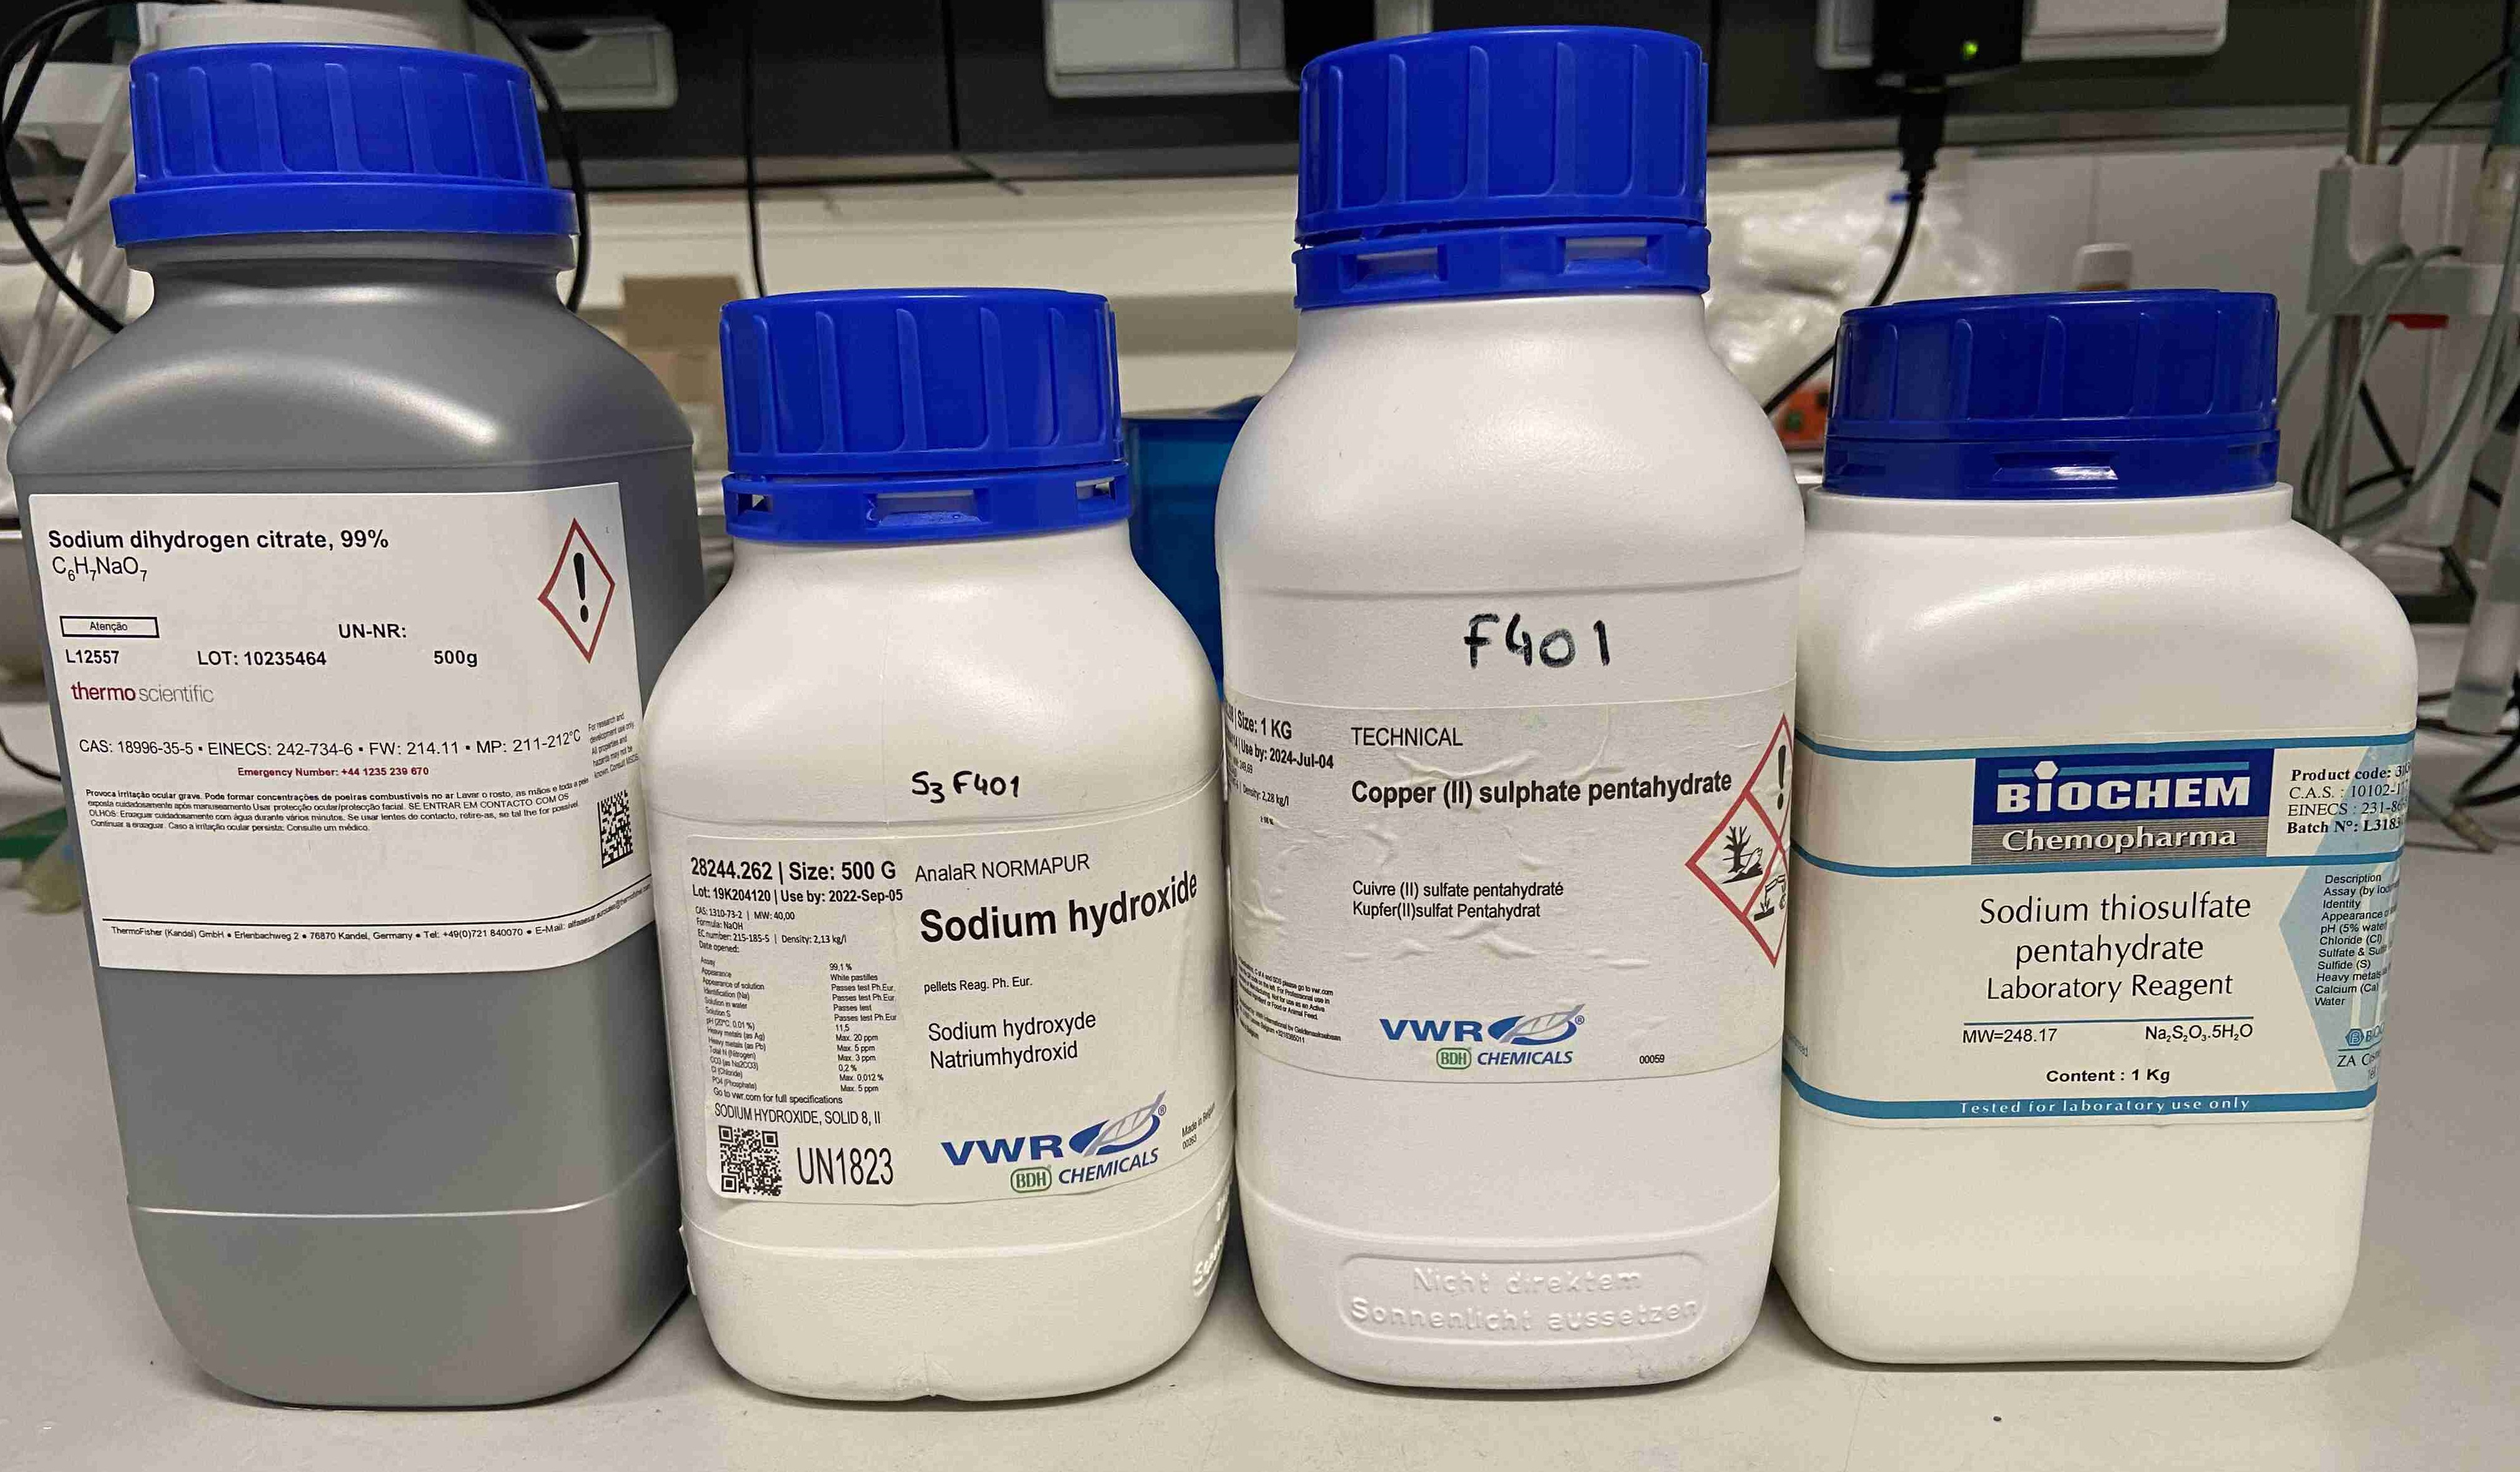
\includegraphics[width=0.9\linewidth]{figures/reagentes lixiviação citrato}
    \caption{Reagentes utilizados na lixiviação (citrato).}
    \label{fig:reagentes-lix-citrato}
\end{marginfigure}

A lixiviação será feita com uma razão sólido líquido de 1 para 5 (S/L = 1/5) e será utilizado 100~g de minerio.

A lixiviação foi efetuada a 90~\graus{}, com uma agitação de 450~rpm, durante 9~horas.
Foi utilizado um reator de borossilicato de 500~mL.

As quantidades de reagentes adicionadas foram as seguintes:
\marginnote{Será preparada uma solução de \hidso{} a 1~M, para ser adicionado pouco a pouco à solução de lixiviação para garantir um pH de 11.}
\begin{itemize}
    \item[-] $\mathrm{m}_{\left[\citratodi{}\right]}$ = 21,41~g;
    \item[-] $\mathrm{m}_{\left[\tsp{}\right]}$ = 24,83~g;
    \item[-] $\mathrm{m}_{\left[\sulfcu{}\right]}$ = 12,48~g.
\end{itemize}

Num gobelé, foi medida a massa de citrato de sódio di-hidratado (21,41~g), a massa de tiossulfato de sódio penta-hidratado (24,83~g) e a massa de sulfato de cobre penta-hidratado (12,48~g) que vão ser utilizados.
Num balão volumétrico de 500~mL foi medido o volume de água destilada de forma a respeitar a relação sólido líquido (500~mL).
Colocou-se um pouco dessa água num gobelé com os reagentes e agitou-se com uma vareta de vidro, de forma a dissolver os reagentes e homogeneizar a solução.

Uma vez dissolvidos os reagentes, foi medida a massa de minério a ser lixiviado (100~g), da amostra \texttt{A08.2}.
O minério foi colocado no reator de borossilicato com 4~aberturas, montou-se o agitador mecânico e colocou-se a solução de lixiviação com os reagentes dissolvidos no reator.
Definiu-se uma rotação de 450~rpm e deu-se início à lixiviação às 10h15.
Passado 2~minutos, mediu-se o pH (1,704).

Adicionou-se 2,5~mL de \hidso{} a 1~M com uma pipeta de 1~mL. 
\textbf{Não houve alterações no valor de pH.}

\marginnote{Após se ter adicionado uma quantidade significativa de \hidso{} a diferentes concentrações e não se ter verificado alterações no valor de pH, decidiu-se continuar com a lixiviação com um pH ácido (cerca de 1,7) para não alterar mais a relação sólido líquido.}

Preparou-se uma solução de \hidso{} a 5~M, adicionou-se 22~gotas com uma pipeta \emph{Pasteur}.
\textbf{Não houve alterações no valor de pH.}

Preparou-se uma solução de \hidso{} a 10~M, adicionou-se 14~gotas com uma pipeta \emph{Pasteur}.
\textbf{Não houve alterações no valor de pH.}

Foi-se medindo o pH de hora em hora.
O valor de pH não subiu nem desceu durante as 9~horas de lixiviação, manteve-se sempre perto de 1,7.

No fim das 9~horas de lixiviação, mediu-se novamente o pH (1,633).
De seguida, montou-se o sistema de filtragem, composto por um filtro de Büchner, um Kitasato, uma bomba de vácuo e um papel de filtro.
Filtrou-se e mediu-se o volume do licor de lixiviação - 500~mL.

O resíduo sólido filtrado foi lavado com 250~mL de água\sidenote{Relação sólido líquido para a lavagem, S/L = 1/2,5.}.
Colocou-se o resíduo de novo no reator, adicionou-se 250~mL de água destilada e ligou-se o agitador, deixando-se a lavar durante 30~minutos com uma velocidade de agitação de 450~rpm.

Após os 30~minutos, filtrou-se novamente o material agora lavado.
Mediu-se o volume de solução de água de lavagem - 249~mL - e mediu-se o pH - 2,794.

Tanto o licor de lixiviação como a água de lavagem, foram colocados em recipientes de vidro, identificados e armazenados.

O material, já lavado e filtrado, foi colocado numa estufa a 60~\graus{} secar durante 8~horas. 
Deixou-se dentro da estufa durante o fim de semana.

\begin{marginfigure}
    \centering
    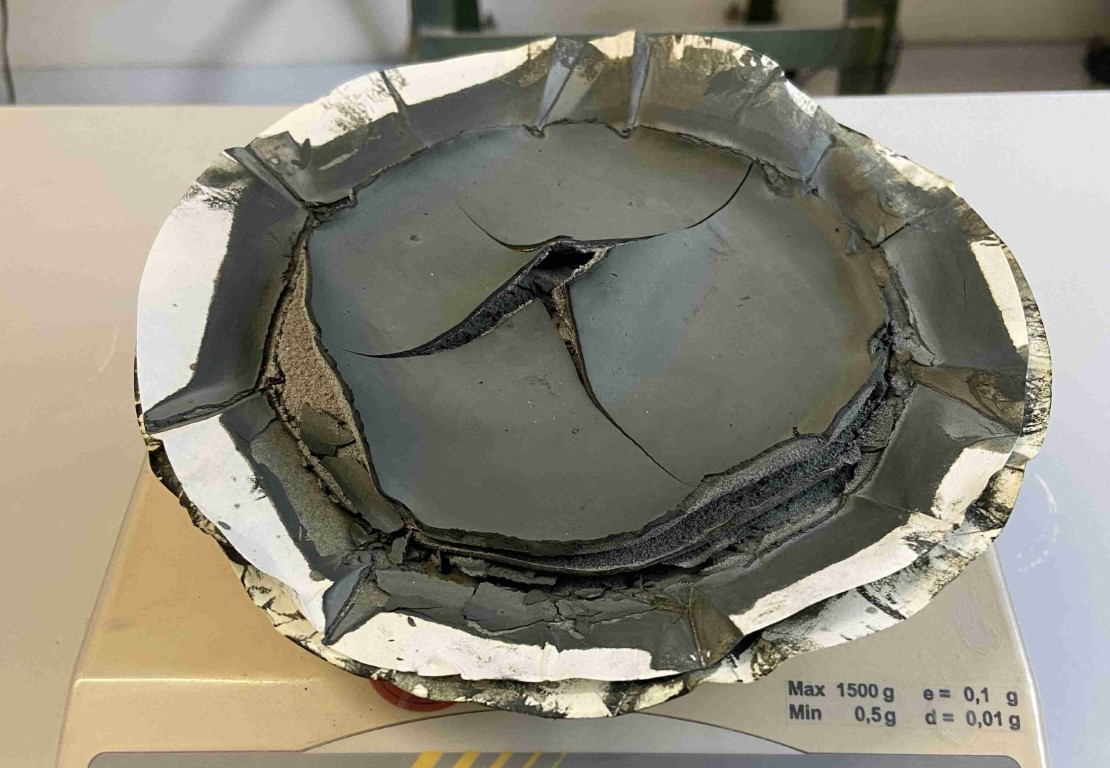
\includegraphics[width=0.9\linewidth]{figures/Resíduo Sólido Lixiviação Citrato}
    \caption{Resíduo sólido da lixiviação seco (citrato).}
    \label{fig:residuo-solido-lix-citrato}
\end{marginfigure}

Após estar seco (Figura~\ref{fig:residuo-solido-lix-citrato}), mediu-se a massa - 90,21~g (já a descontar o vidro de relógio e o papel de filtro). 
Reservou-se.

O resíduo sólido será submetido a digestão ácida para análise posterior na absorção atómica.

\newthought{Concentrações em \ce{Au}:} Licor de lixiviação - 1,00~mg/L; água de lavagem - 0,110~mg/L; resíduo (média) - 5,11~ppm.

\hrulefill

%%%%%%%%%%%%%%%%%%%%%%%%%%%%%%%%%%%%%%%%%%%%%%%%%%%%%%%%

\newday{Digestões ácidas dos resíduos de lixiviação - Citrato}

Após se realizar as digestões ácidas\sidenote{O procedimento para a digestão ácida foi o mesmo realizado no dia~\nameref{day:8-novembro-2024}.} do resíduo sólido lixiviado com citrato, analisou-se na absorção atómica.

Após a análise na \emph{AAS}, obteve-se a Tabela~\ref{tab:aas-concentracao-au-res-citrato} referente às concentrações em \ce{Au} no resíduo de lixivição com Citrato:

\begin{table}[!ht]
    \centering
    \begin{tabularx}{\textwidth}{@{}lCCC@{}}
        \toprule
        \textbf{Amostra} & \textbf{Absorção} & \textbf{Conc. (mg/L)} & \textbf{Teor \ce{Au} (ppm)}\\ \midrule
        \textbf{Dig. 1}  & 0,03469 & 0,96 & 4,7974 \\
        \textbf{Dig. 2}  & 0,03751 & 1,04 & 5,2026 \\
        \textbf{Dig. 3}  & 0,04389 & 1,22 & 6,1193 \\
        \textbf{Dig. 4}  & 0,03482 & 0,96 & 4,8161 \\
        \textbf{Dig. 5}  & 0,03338 & 0,92 & 4,6092 \\ \bottomrule
    \end{tabularx}
    \caption{Concentração em \ce{Au} no resíduo de lixiviação com Citrato.}
    \label{tab:aas-concentracao-au-res-citrato}
\end{table}

Da absorção atómica também se determinou a concentração em \ce{Au} do licor de lixviação (\textbf{1,00~mg/L}) e da água de lavagem (\textbf{0,11~mg/L}).

\hrulefill

%%%%%%%%%%%%%%%%%%%%%%%%%%%%%%%%%%%%%%%%%%%%%%%%%%%%%%%%

\section*{Resultados das Lixiviações Preliminares}

\subsection*{Tiossulfato}

Após analisar o licor de lixiviação, a água de lavagem e as digestões ácidas dos resíduos sólidos da lixiviação na absorção atómica, obteve-se os seguintes resultados para a primeira lixiviação realizada com Tiossulfato (dia~\nameref{day:15-novembro-2024}):

\begin{table}[!ht]
    \centering
    \begin{tabularx}{\textwidth}{@{}CCCC@{}}
        \toprule
        \textbf{Teor Alim. (ppm)} & \textbf{Rendimento fase líquida} & \textbf{Rendimento fase sólida} & \textbf{Teor Resíduo (ppm)} \\ \midrule
        9,87 & 36,54~\% & -0,71~\% & 9,94 \\ \bottomrule                  
    \end{tabularx}
    \caption{Teor da alimentação original (Tiossulfato).}
    \label{tab:original-grade-feed-tiossulfato}
\end{table}

O teor em \ce{Au} do resíduo de lixiviação é superior ao teor em \ce{Au} da alimentação.
Isto indica que houve erros, ou na digestão ácida da alimentação, ou na amostragem do material.

Como o ouro está presente numa quantidade muito pequena, a probabilidade de erros durante a amostragem é elevada. 
Provavelmente, durante a separação, a parte da amostra que continha menos \ce{Au} foi utilizada na digestão ácida. 

Aliás, isto é ainda mais comprovado pelo facto de que o saco \texttt{A08.3} foi utilizado para a lixiviação com Tiossulfato e para a digestão ácida da alimentação. 
Ou seja, os valores deveriam ser iguais, visto que se trata do mesmo material.

Dessa forma, calculou-se o teor da alimentação de acordo com os valores do teor em \ce{Au} do resíduo de lixiviação e do licor e água de lavagem, obtendo-se a Tabela~\ref{tab:compatibalized-grade-feed-tiossulfato}.

\begin{table}[!ht]
    \centering
    \begin{tabularx}{\textwidth}{@{}CC@{}}
        \toprule
        \textbf{Teor Alim. compatiblizado (ppm)} & \textbf{Rendimento fase líquida} \\ \midrule
        13,55 & 26,62~\% \\ \bottomrule                  
    \end{tabularx}
    \caption{Teor da alimentação compatibilizado (Tiossulfato).}
    \label{tab:compatibalized-grade-feed-tiossulfato}
\end{table}

O rendimento compatibilizado é muito baixo (26,62~\%). 
Deverão ser averiguados os fatores que podem ter influenciado os resultados obtidos e desenvolver um plano de lixiviação que permita obter melhores redimentos.

\hrulefill

\subsection*{Tioureia}

Após analisar o licor de lixiviação, a água de lavagem e as digestões ácidas dos resíduos sólidos da lixiviação na absorção atómica, obteve-se os segunites resultados para a primeira lixiviação realizada com Tioureia (dia~\nameref{day:22-novembro-2024}):

\begin{table}[!ht]
    \centering
    \begin{tabularx}{\textwidth}{@{}CCCC@{}}
        \toprule
        \textbf{Teor Alim. (ppm)} & \textbf{Rendimento fase líquida} & \textbf{Rendimento fase sólida} & \textbf{Teor Resíduo (ppm)} \\ \midrule
        9,87 & 59,98~\% & 11,75~\% & 8,71 \\ \bottomrule                  
    \end{tabularx}
    \caption{Teor da alimentação original (Tioureia).}
    \label{tab:original-grade-feed-tioureia}
\end{table}

Realizou-se também a compatibilização do teor da alimentação, tendo em conta os valores de teor em \ce{Au} obtidos pelas análises do licor, da água de lavagem e do resíduo sólido da lixiviação:

\begin{table}[!ht]
    \centering
    \begin{tabularx}{\textwidth}{@{}CC@{}}
        \toprule
        \textbf{Teor Alim. compatiblizado (ppm)} & \textbf{Rendimento fase líquida} \\ \midrule
        14,63 & 40,47~\% \\ \bottomrule                  
    \end{tabularx}
    \caption{Teor da alimentação compatibilizado (Tioureia).}
    \label{tab:compatibalized-grade-feed-tioureia}
\end{table}

Neste ensaio já se observa rendimentos mais elevados, no entanto continuam a ser inferiores aos rendimentos obtidos no artigo científico\cite{innovative_thiourea_1998} utilizado para elaborar o procedimento.
Obtivemos um rendimento (compatibilizado) de 40,47~\%, enquanto que no artigo obtêm rendimentos de 85~\%.

Existem vários fatores que se pensa terem influenciado estes resultados.
O primeiro é que não se tem a certeza se a concentração de ferro se refere à concentração de \ce{Fe} ou de \ce{Fe2(SO4)3}.

O segundo é que se suspeita de uma quantidade de reagente insuficiente. 
Pode ser que a quantidade de tioureia utilizada seja insuficiente para lixiviar o material. 
Uma solução será aumentar a quantidaded de Tioureia adicionada. 

Outro fator pode ser a temperatura.
No artigo são realizadas lixiviações a diferentes temperaturas (20~\graus{}, 40~\graus{} e 60~\graus{}).
Apesar de estar claro no artigo que a lixiviação a diferentes temperaturas não apresentam aumentos significativos no rendimento.

\hrulefill

\subsection*{Bromo}

Após analisar o licor de lixiviação, a água de lavagem e as digestões ácidas dos resíduos sólidos da lixiviação na absorção atómica, obteve-se os seguintes resultados para a primeira lixiviação realizada com Brometo de sódio (dia~\nameref{day:27-novembro-2024}).

\begin{table}[!ht]
    \centering
    \begin{tabularx}{\textwidth}{@{}CCCC@{}}
        \toprule
        \textbf{Teor Alim. (ppm)} & \textbf{Rendimento fase líquida} & \textbf{Rendimento fase sólida} & \textbf{Teor Resíduo (ppm)} \\ \midrule
        9,87 & 29,85~\% & 7,53~\% & 9,127 \\ \bottomrule                  
    \end{tabularx}
    \caption{Teor da alimentação original (Brometo de Sódio).}
    \label{tab:original-grade-feed-bromo}
\end{table}

Realizou-se também a compatibilização do teor da alimentação, tendo em conta os valores de teor em \ce{Au} obtidos pelas análises do licor, da água de lavagem e do resíduo sólido da lixiviação:

\begin{table}[!ht]
    \centering
    \begin{tabularx}{\textwidth}{@{}CC@{}}
        \toprule
        \textbf{Teor Alim. compatiblizado (ppm)} & \textbf{Rendimento fase líquida} \\ \midrule
        10,79 & 15,41~\% \\ \bottomrule                  
    \end{tabularx}
    \caption{Teor da alimentação compatibilizado (Brometo de Sódio).}
    \label{tab:compatibalized-grade-feed-bromo}
\end{table}

Novamente, observa-se valores de rendimento muito baixos comparados aos obtidos no artigo científico\cite{bromo_2018} seguido.
Obteve-se um rendimento (compatibilizado) de 15,41~\%, enquanto que no artigo obtêm rendimentos de 73~\%.

Relativamente a fatores que possam ter influenciado os valores obtidos, coloca-se a hipótese de fuga de bromo quando se realizou a medição do pH (apesar de não se ter verificado ``vapor laranja'' a sair do reator de borossilicato).
Outra hipótese pode ser a fuga gradual de bromo pela abertura entre a rolha e o agitador mecânico.
Mesmo tendo sido utilizada uma rolha nova, verificou-se que com a rotação do agitador, a abertura da rolha foi gradualmente aumentando.
Verificou-se, também, resíduo que escorreu pela parte de fora do reator quando se retirou este do banho maria para realizar a filtração.
Não se sabe\sidenote{Apenas a colocar hipóteses.} como é que foi possível a fuga de qualquer tipo de material (gás ou líquido), tendo-se selado fortemente o reator de borossilicato.

\hrulefill

\subsection*{Citrato}

Após analisar o licor de lixiviação, a água de lavagem e as digestões ácidas dos resíduos sólidos da lixiviação na absorção atómica, obteve-se os seguintes resultados para a primeira lixiviação realizada com Citrato (dia~\nameref{day:29-novembro-2024}).

\begin{table}[!ht]
    \centering
    \begin{tabularx}{\textwidth}{@{}CCCC@{}}
        \toprule
        \textbf{Teor Alim. (ppm)} & \textbf{Rendimento fase líquida} & \textbf{Rendimento fase sólida} & \textbf{Teor Resíduo (ppm)} \\ \midrule
        9,87 & 53,43~\% & 48,24~\% & 5,11 \\ \bottomrule                  
    \end{tabularx}
    \caption{Teor da alimentação original (Citrato).}
    \label{tab:original-grade-feed-citrato}
\end{table}

Realizou-se também a compatibilização do teor da alimentação, tendo em conta os valores de teor em \ce{Au} obtidos pelas análises do licor, da água de lavagem e do resíduo sólido da lixiviação:

\begin{table}[!ht]
    \centering
    \begin{tabularx}{\textwidth}{@{}CC@{}}
        \toprule
        \textbf{Teor Alim. compatiblizado (ppm)} & \textbf{Rendimento fase líquida} \\ \midrule
        15,78 & 67,63~\% \\ \bottomrule                  
    \end{tabularx}
    \caption{Teor da alimentação compatibilizado (Citrato).}
    \label{tab:compatibalized-grade-feed-citrato}
\end{table}

No caso do citrato, surpreendentemente, obtivemos rendimentos superiores aos outros três ensaios.
Surpreendentemente porque devido ao que ocorreu durante o ensaio\sidenote{Alteração da cor da polpa para preto. Ver resíduo sólido da lixiviação, Figura~\ref{fig:residuo-solido-lix-citrato}.}, esperava-se piores resultados.
Supõe-se que a alteração da cor durante a lixiviação seja devido à presença de reagentes utilizados no tratamento anterior a que o minério foi sujeito\sidenote{O minério da mina do Numão com que se está a trabalhar é um pré-concentrado que foi submetido a tratamentos hidrometalúrgicos anteriores, como a flutuação.}.
No entanto, foi o ensaio que até agora apresentou melhores resultados relativamente ao rendimento (67,63~\%).

De notar que o rendimento de 67,63~\% obtido é para o teor da alimentação compatibilizado, que tem um valor de 15,78~ppm, consideravelmente superior ao teor da alimentação original (9,87~ppm).
Possivelmente, a amostra utilizada (\texttt{A08.2}) na lixiviação com citrato tenha uma concentração em \ce{Au} superior às restantes. 
Sobrou cerca de 159~g de material dessa amostra que não foi lixiviado.
Será prudente realizar uma outra lixiviação com citrato dessa mesma amostra, para confirmar os resultados obtidos e verificar se ocorre novamente a alteração da cor.